\documentclass[11pt]{article}

\usepackage[portuguese]{babel}
\usepackage[utf8]{inputenc}
\usepackage{amsmath}
\usepackage{graphicx}
\usepackage{float}
\usepackage{subfig}
\usepackage{fixltx2e}
\usepackage[bottom]{footmisc}
\usepackage{color}
\usepackage{xargs}                      % Use more than one optional parameter in a new commands
\usepackage[pdftex,dvipsnames]{xcolor}  % Coloured text etc.
\usepackage[colorinlistoftodos,prependcaption,textsize=tiny]{todonotes}
\newcommandx{\unsure}[2][1=]{\todo[linecolor=red,backgroundcolor=red!25,bordercolor=red,#1]{#2}}
\newcommandx{\change}[2][1=]{\todo[linecolor=blue,backgroundcolor=blue!25,bordercolor=blue,#1]{#2}}
\newcommandx{\info}[2][1=]{\todo[linecolor=OliveGreen,backgroundcolor=OliveGreen!25,bordercolor=OliveGreen,#1]{#2}}
\newcommandx{\improvement}[2][1=]{\todo[linecolor=Plum,backgroundcolor=Plum!25,bordercolor=Plum,#1]{#2}}
\newcommandx{\thiswillnotshow}[2][1=]{\todo[disable,#1]{#2}}
\usepackage[font=footnotesize]{caption}

\numberwithin{equation}{section}

\linespread{1.3}
\usepackage{indentfirst}
\usepackage[top=2cm, bottom=2cm, right=2.25cm, left=2.25cm]{geometry}
\addto\captionsportuguese{\renewcommand{\contentsname}{Índice}}

\begin{document}

\begin{titlepage}
\begin{center}

\hfill \break
\hfill \break


\includegraphics[width=0.3\textwidth]{./logo}~\\[1cm]

\textsc{\LARGE Instituto Superior Técnico}\\[0.25cm]
\textsc{\Large Mestrado Integrado em Engenharia Electrotécnica e de Computadores}\\[1.8cm]
\textsc{\huge Sistemas Integrados Analógicos}\\[0.25cm]

{\huge \bfseries \textit{Design} de um Amplificador \\[1cm]}

\begin{tabular}{ l l }
João Bernardo Sequeira de Sá & \hspace{2mm} n.º 68254 \\
Maria Margarida Dias dos Reis & \hspace{2mm} n.º 73099 \\
Nuno Miguel Rodrigues Machado & \hspace{2mm} n.º 74236
\end{tabular}

\vfill

{\large Lisboa, 31 de Maio de 2015} 

\end{center}
\end{titlepage}

\pagenumbering{gobble}
\clearpage

\tableofcontents
\pagebreak

\clearpage
\pagenumbering{arabic}

\section{Introdução}

Pretende-se projectar um amplificador \textit{folded cascode} CMOS OTA de dois andares de acordo com as especificações da seguinte tabela.

\begin{table}[H]
	\centering
	\caption{Características do amplificador a projectar.}
	\vspace{-1.5mm}
	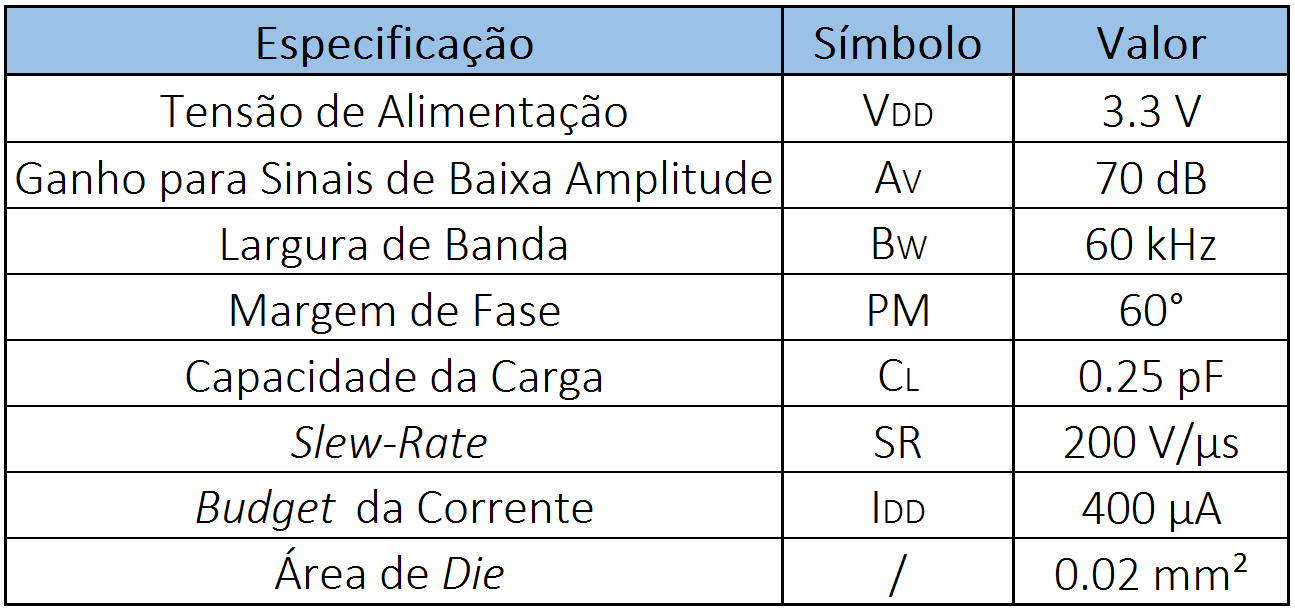
\includegraphics[keepaspectratio=true, scale=0.45]{teoricas/tabela1}
	\label{tab:tab1}
\end{table}

O circuito de ponto de partida para a realização do projecto é apresentado de seguida.

\begin{figure}[H]
	\centering
	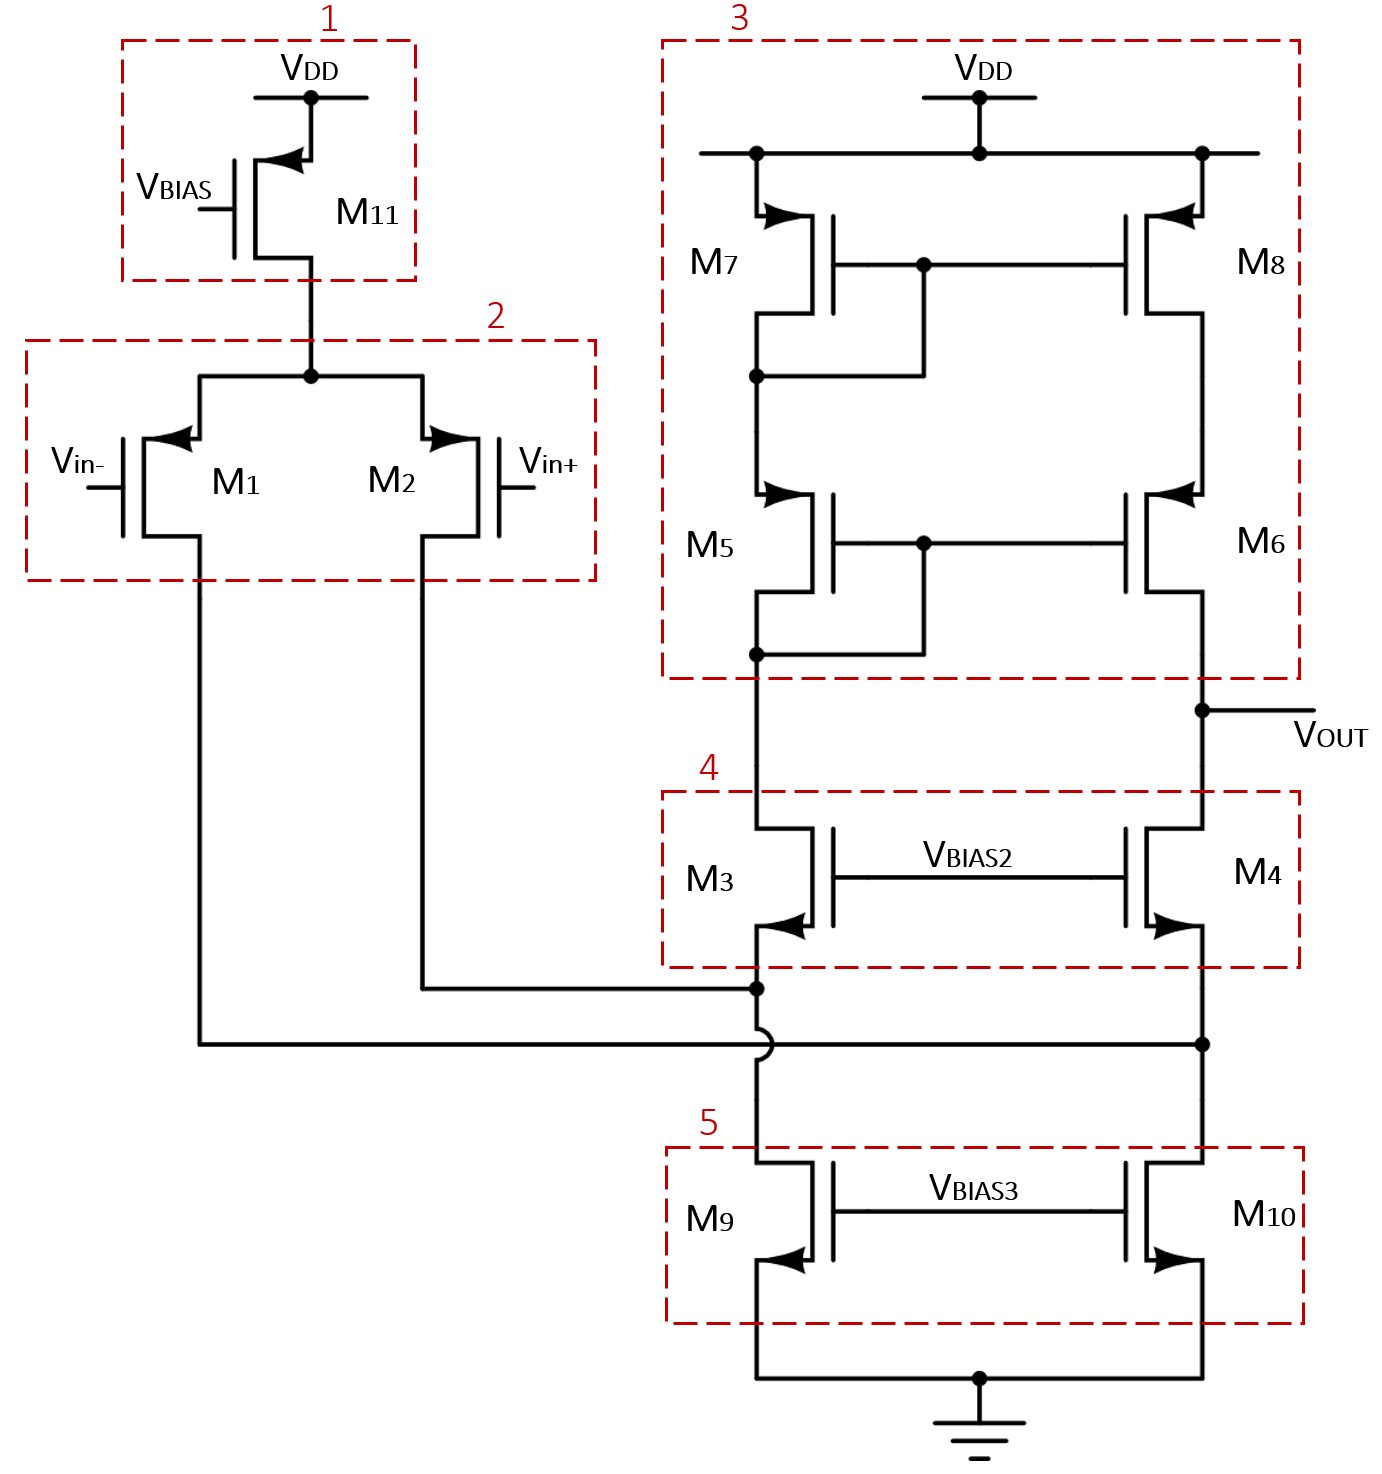
\includegraphics[keepaspectratio=true, scale=0.50]{teoricas/circuito1}
	\vspace{-0.5em}
	\caption{Circuito do amplificador a projectar.}
	\vspace{-0.8em}
\end{figure} 

\section{Adenda ao \textit{Middle Target}}

Esta secção foi acrescentada ao relatório final no intuito de corrigir os resultados obtidos e apresentados no relatório anterior, o do \textit{middle target}. Como referenciado, pretende-se projectar um amplificador \textit{folded cascode} CMOS OTA de dois andares de acordo com as especificações da Tabela \ref{tab:tab1}.

\subsection{Detecção dos erros} 

Foram identificados vários erros no relatório intermédio que comprometem os resultados apresentados anteriormente. A primeira correcção foi referente ao \textit{schematic} do \textit{testbench} que permite simular o circuito em testes de resposta AC. Foi colocado um \textit{switch} que simula a bobine - provoca um circuito aberto para um regime AC e curto-circuito para um regime DC. Foi também alterada a amplitude do sinal de entrada de 3.3 V para 1.6 V, sendo que esta alteração garante que os transístores não saem da saturação. De seguida pode-se comparar o novo \textit{testbench} com o anterior.

\begin{figure}[H]
	\centering
	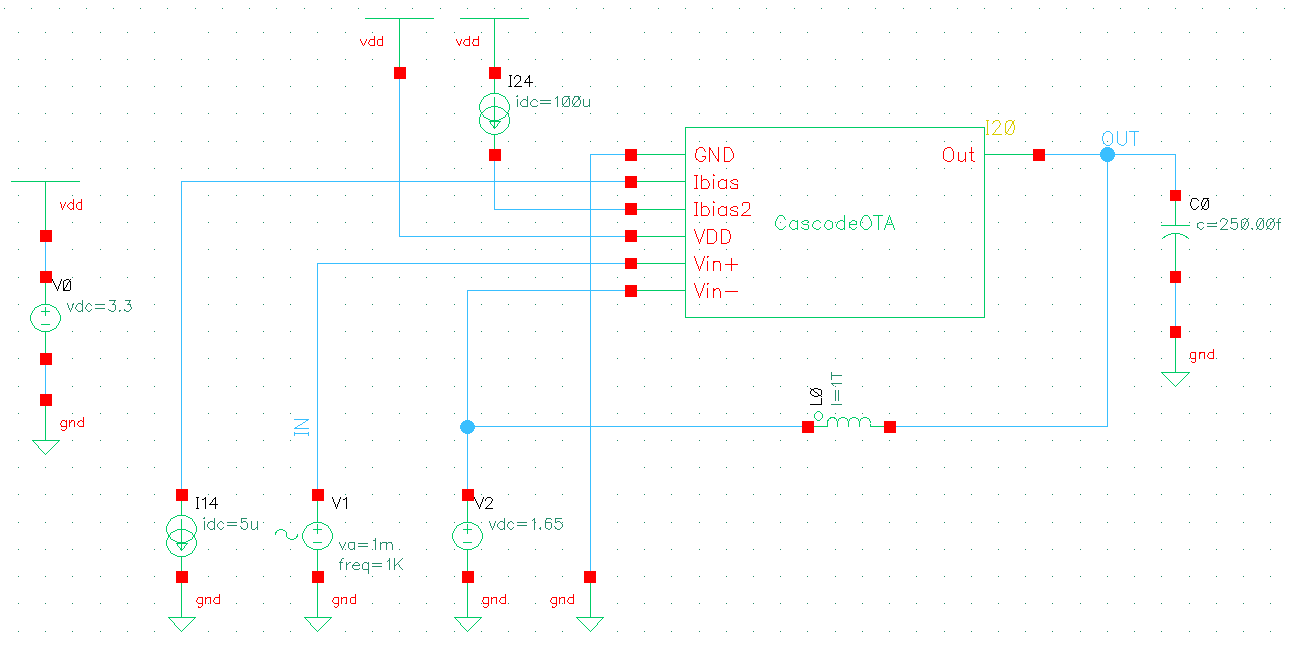
\includegraphics[keepaspectratio=true, scale=0.60]{exps/TBac}
	\vspace{-0.5em}
	\caption{\textit{Schematic} do \textit{testbench} anterior que permite simular o circuito em testes de resposta AC.}
	\vspace{-0.8em}
\end{figure} 

\begin{figure}[H]
	\centering
	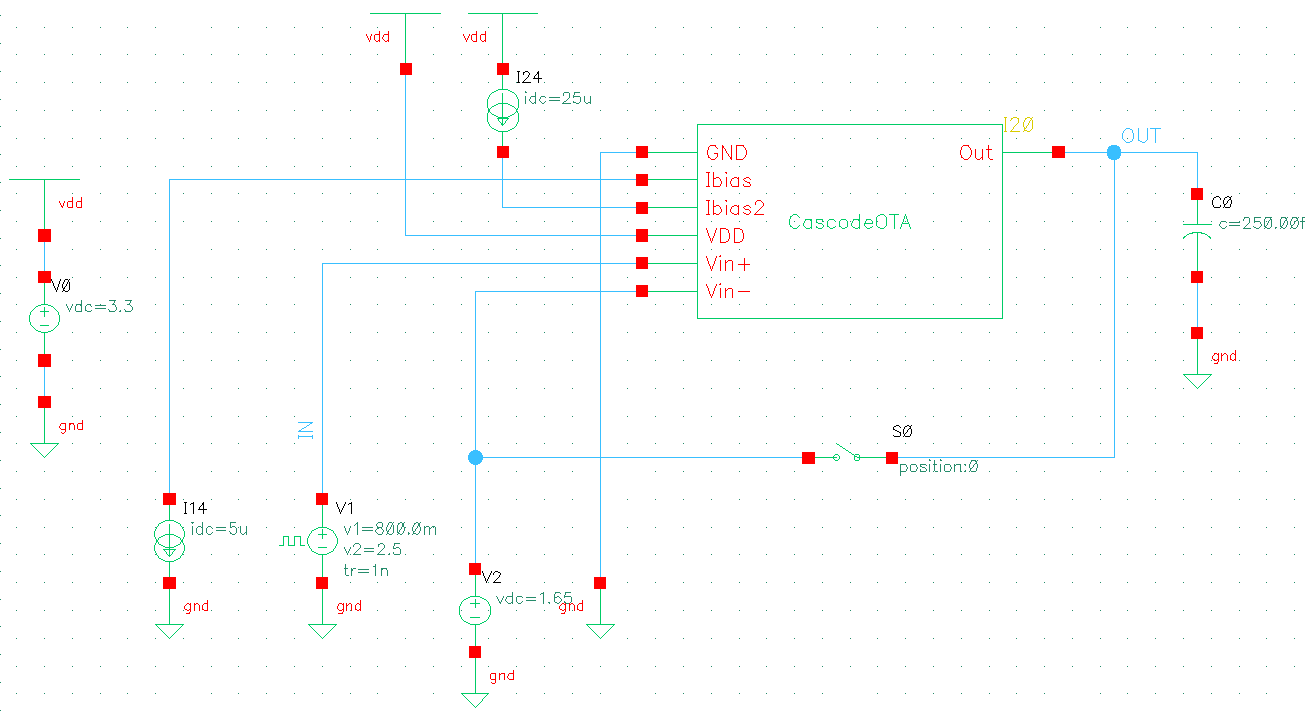
\includegraphics[keepaspectratio=true, scale=0.50]{exps/testebenchantigo}
	\vspace{-0.5em}
	\caption{\textit{Schematic} do novo \textit{testbench} que permite simular o circuito em testes da \textit{slew-rate} e de resposta transiente, DC e AC.}
	\vspace{-0.8em}
\end{figure} 

Outro erro identificado é referente ao cálculo da \textit{slew-rate}. No relatório intermédio, o resultado da \textit{slew-rate} era relativo só ao flanco de descida, sendo necessário demonstrar para os dois flancos - subida (equação 2.1) e descida (equação 1.2). 

\vspace{-3mm}
\begin{equation}
	\text{slewRate} (\text{VT("/OUT")} \:\: 1 \:\: \text{nil} \:\: 2 \:\: \text{nil} \:\: 10 \:\: 90 \:\: \text{nil} \:\: "\text{time}")
\end{equation}

\vspace{-3mm}
\begin{equation}
	\text{slewRate} (\text{VT("/OUT")} \:\: 2 \:\: \text{nil} \:\: 1 \:\: \text{nil} \:\: 10 \:\: 90 \:\: \text{nil} \:\: "\text{time}")
\end{equation}

A equação \texttt{slewRate} é obtida com recurso à calculadora do Cadence, escolhendo o sinal pretendido, que, neste caso, é a saída do \textit{cascode} OTA, \texttt{VT("/OUT")}. De seguida escolhe-se a posição inicial e final para o cálculo da \textit{slew-rate} - foi definido que para o flanco de descida começa-se a calcular desde 2 V até 1 V e no flanco de subida o cálculo é o inverso, de 1 V até 2 V. O intervalo anteriormente referido foi escolhido de forma a calcular a \textit{slew-rate} na zona onde os transístores se encontram na saturação.

\subsection{Correcção do dimensionamento}

Com os erros anteriormente referidos corrigidos, o circuito apresentado na entrega intermédia falhava em algumas especificações: ganho para sinais de baixa amplitude, margem de fase e largura de banda. Na secção seguinte apresenta-se os resultados das simulações de Monte Carlo e \textit{corners}.

Com o intuito de corrigir as dimensões, partiu-se de um critério inicial - obter transístores de dimensões mais reduzidas e manter o rácico $W/L$ obtido no relatório anterior. Em primeiro lugar, verificou-se que com a nova expressão do cálculo da \textit{slew-rate} obtém-se valores mais elevados, o que significa que se pode reduzir as dimensões dos transístores M\textsubscript{9} e M\textsubscript{10}. 

De seguida pretendeu-se melhorar a margem de fase e, analisando o resultado das especificações pretendidas, verificou-se que era necessário aumentar a largura de banda de forma a obter uma margem de fase melhor sem alterar significativamente os resultados das outras especificações. Começou-se por analisar as dimensões das capacidades do circuito e verificou-se que a capacidade referente aos transístores M\textsubscript{7} e M\textsubscript{8} é a capacidade que mais influencia a margem de fase. Mas, como já foi referido no relatório anterior, os transístores M\textsubscript{7} e M\textsubscript{8} também afectam o ganho e a largura de banda, como se pode ver pelas expressões seguintes. 

\vspace{-3mm}
\begin{equation}
A_{v} = g_{m_1} R_o =  g_{m_1}\left[\left(g_{m_4}r_{o_4}\left(r_{o_2}//r_{o_{10}}\right)\right)//\left(g_{m_6}r_{o_6}r_{o_8}\right)\right];
\end{equation}
\vspace{-2mm}
\begin{equation}
f_{p} = \frac{1}{2\pi C_L R_o} = \frac{1}{2\pi C_L \left[\left(g_{m_4}r_{o_4}\left(r_{o_2}//r_{o_{10}}\right)\right)//\left(g_{m_6}r_{o_6}r_{o_8}\right)\right]};
\end{equation} 

\vspace{2mm}
Assim sendo, e analisando as expressões decidiu-se inicialmente diminuir as dimensões dos transístores M\textsubscript{7} e M\textsubscript{8}, o que fez aumentar a largura de banda como também a margem de fase. Com o intuito de melhorar as especificações obtidas diminui-se as dimensões dos transístores M\textsubscript{3} e M\textsubscript{4} até atingir uma dimensão de $L$ miníma de 0.85 $\mu$m. Como a dimensão $L$ dos transístores M\textsubscript{5} e M\textsubscript{6} é menor que 0.85 $\mu$m, aumentou-se as dimensões com o intuito de manter o critério de um L mínimo de 0.85 $\mu$m.

Com estas alterações consegui-se obter todas a especificações excepto para o ganho de sinais de baixa amplitude. Analisando a expressão anterior do ganho, verifica-se que para aumentar o ganho sem alterar as restantes especificações, seria necessário aumentar o valor de $g_{m_1}$. Como o valor de $g_m$ é directamente proporcional a $I_D$, com aumento de $W$ existe um aumento de $I_D$ e de $g_m$. A expressão seguinte mostra como $W$ influencia $I_D$:

\vspace{-3mm}
\begin{equation}
g_{m} \propto I_{D}= k_P \times \left(\frac{W}{L}\right) \times V_{OD}^2 \times \left(1+\lambda V_{DS}\right).
\end{equation}

Para aumentar o $g_{m_1}$ é necessário alterar o rácio $W/L$, ou seja, o rácio de M\textsubscript{1} e M\textsubscript{2} sofreu um aumento de 132\%, passando de 43 para 100. Não é preocupante esta alteração do valor da transcondutância, não se comprometendo a zona de funcionamento dos transístores pois estes são polarizados externamente.

A polarização do espelho de corrente constituída pelo par M\textsubscript{11\textsubscript{1}} e M\textsubscript{11\textsubscript{2}} através de \texttt{Ibias}. De forma a ter-se um valor baixo para o \textit{budget} da corrente escolheu-se em primeira instância dar-lhe o valor de 5 $\mu$A sendo este multiplicado no espelho de corrente para um valor de 100 

As dimensões dos pares de transístores M\textsubscript{3}/M\textsubscript{4} e  M\textsubscript{9}/ M\textsubscript{10} ficaram definidas à partida, sendo que foi então necessário dimensionar os transístores que iriam ser responsáveis pela sua polarização sendo o critério a corrente de polarização \textit{Ibias2}. Foi então novamente objectivo que esta fosse a mais baixo possível, garantindo o \textit{budget} de corrente. Escolheu-se numa primeira aproximação o valor de 25 $\mu$A, mas após correr as simulações Monte Carlo verificou-se que seria necessário aumentar um pouco este valor ficando o se valor final em 29 $\mu$A. Esta subida foi feita de forma a evitar fazer alterações muito grandes nos transístores M\textsubscript{3}/M\textsubscript{4}, pois tal como este par a corrente \textit{Ibias2} terá ligeiras influências em todos os parâmetros, sendo que se tentou aumentar esta o minimo tentando reduzir também nas alterações necessárias ao par de transístores.
 
Assim, o circuito final relativamente à entrega intermédia é:

\begin{figure}[H]
	\centering
	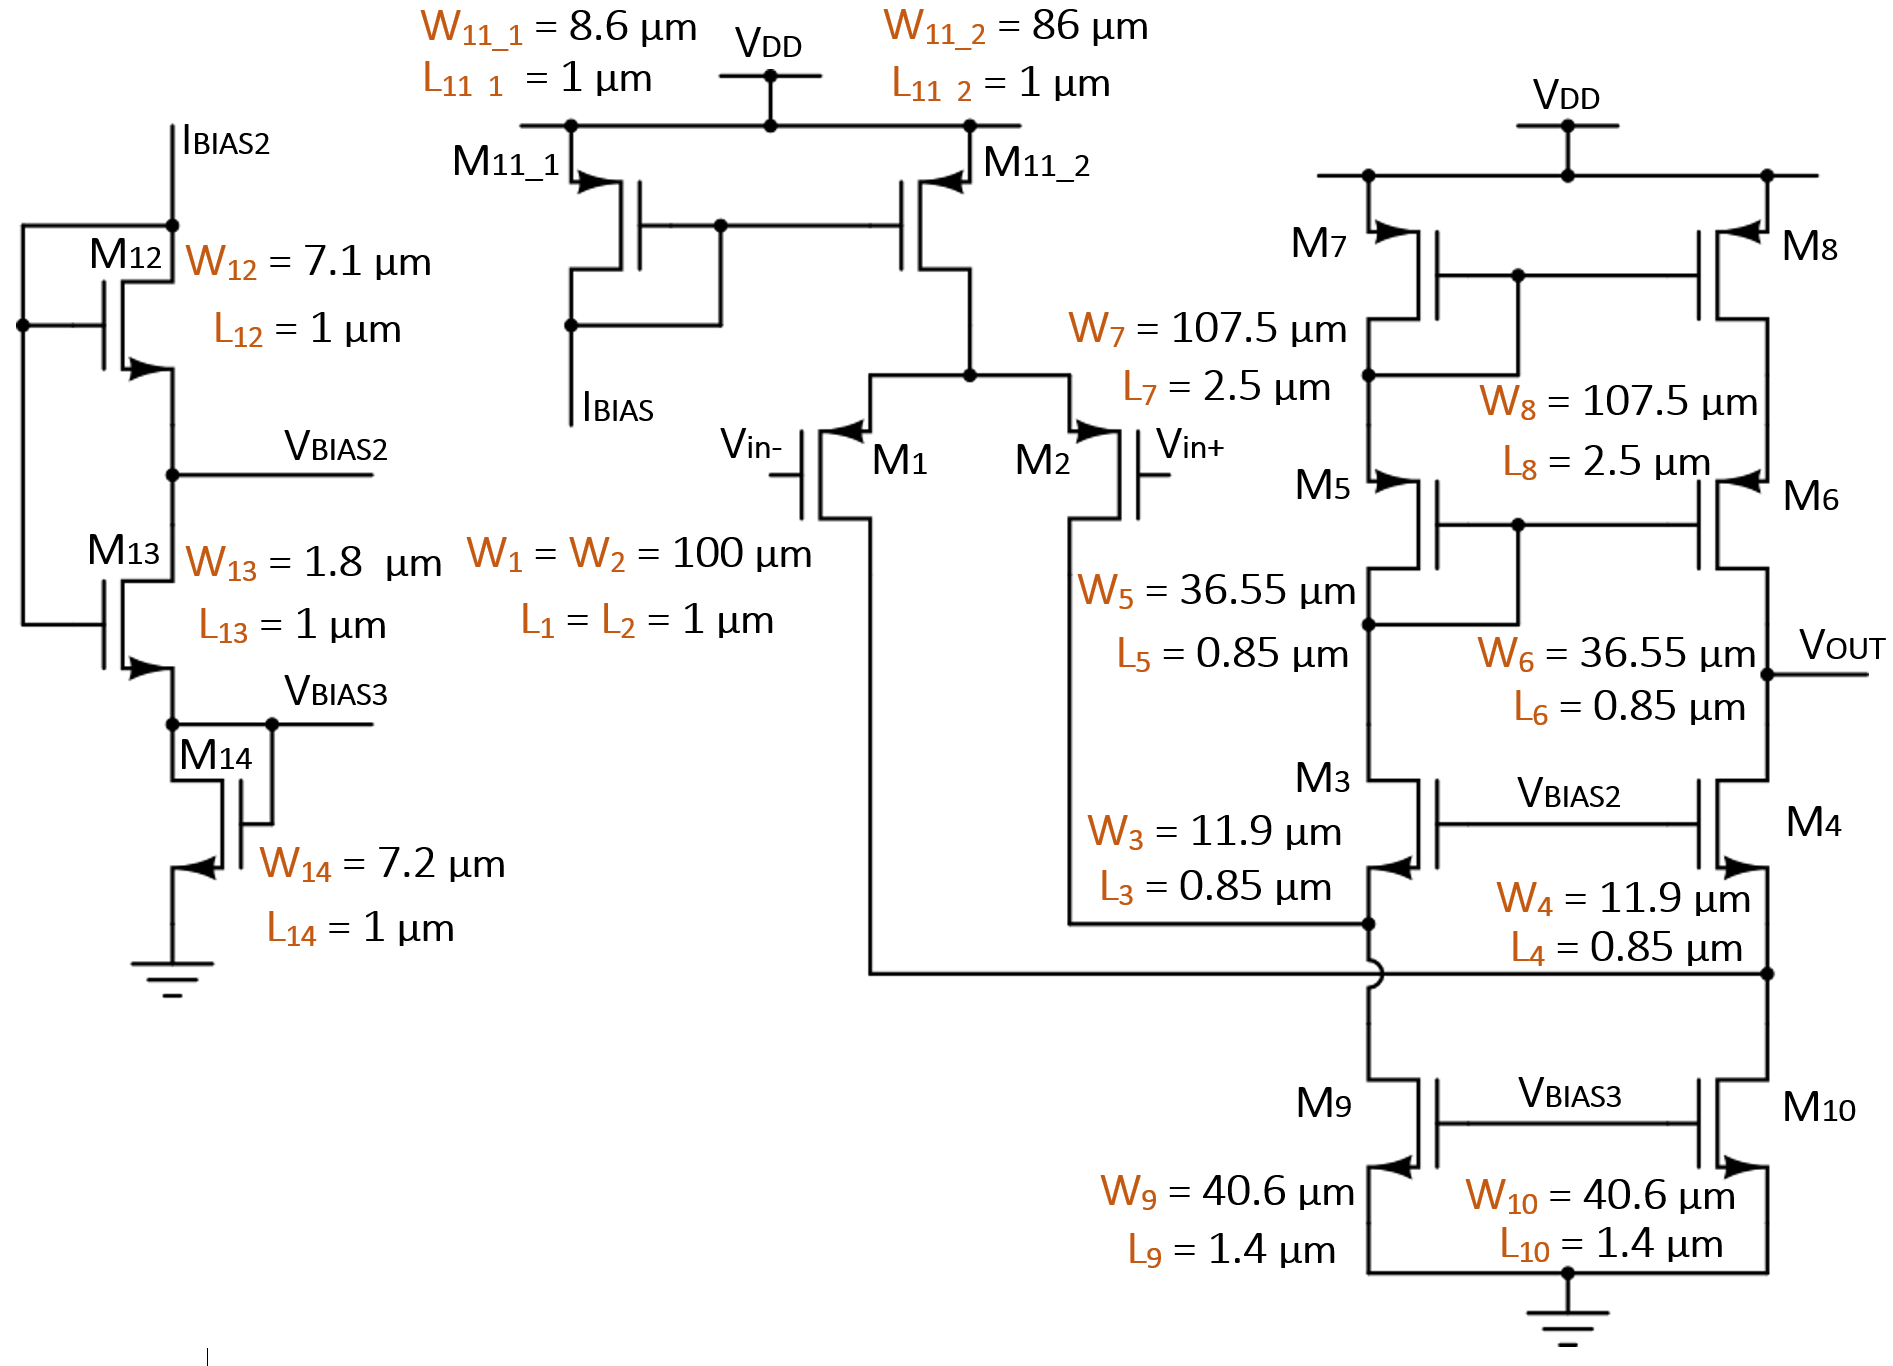
\includegraphics[keepaspectratio=true, scale=0.42]{teoricas/circuitoantesdadiv}
	\vspace{-0.5em}
	\caption{Circuito final da entrega intermédia.}
	\vspace{-0.8em}
	\label{fig:finalint}
\end{figure} 

\begin{table}[H]
	\centering
	\caption{Dimensões dos transístores que constituem o amplificador.}
	\vspace{-1.5mm}
	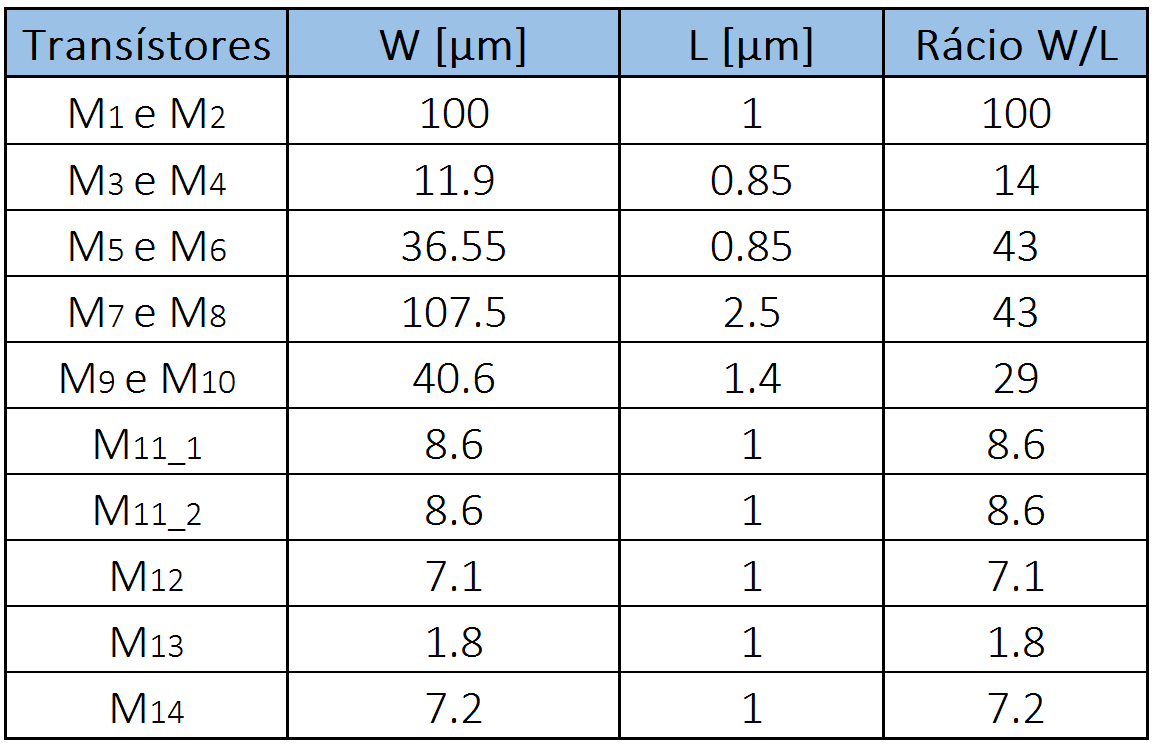
\includegraphics[keepaspectratio=true, scale=0.35]{teoricas/dimensoes1}
\end{table}

Com este circuito as especificações finais obtidas para o circuito com recurso à simulação da Figura 3 são apresentadas na seguinte tabela.

\begin{figure}[H]
	\centering
	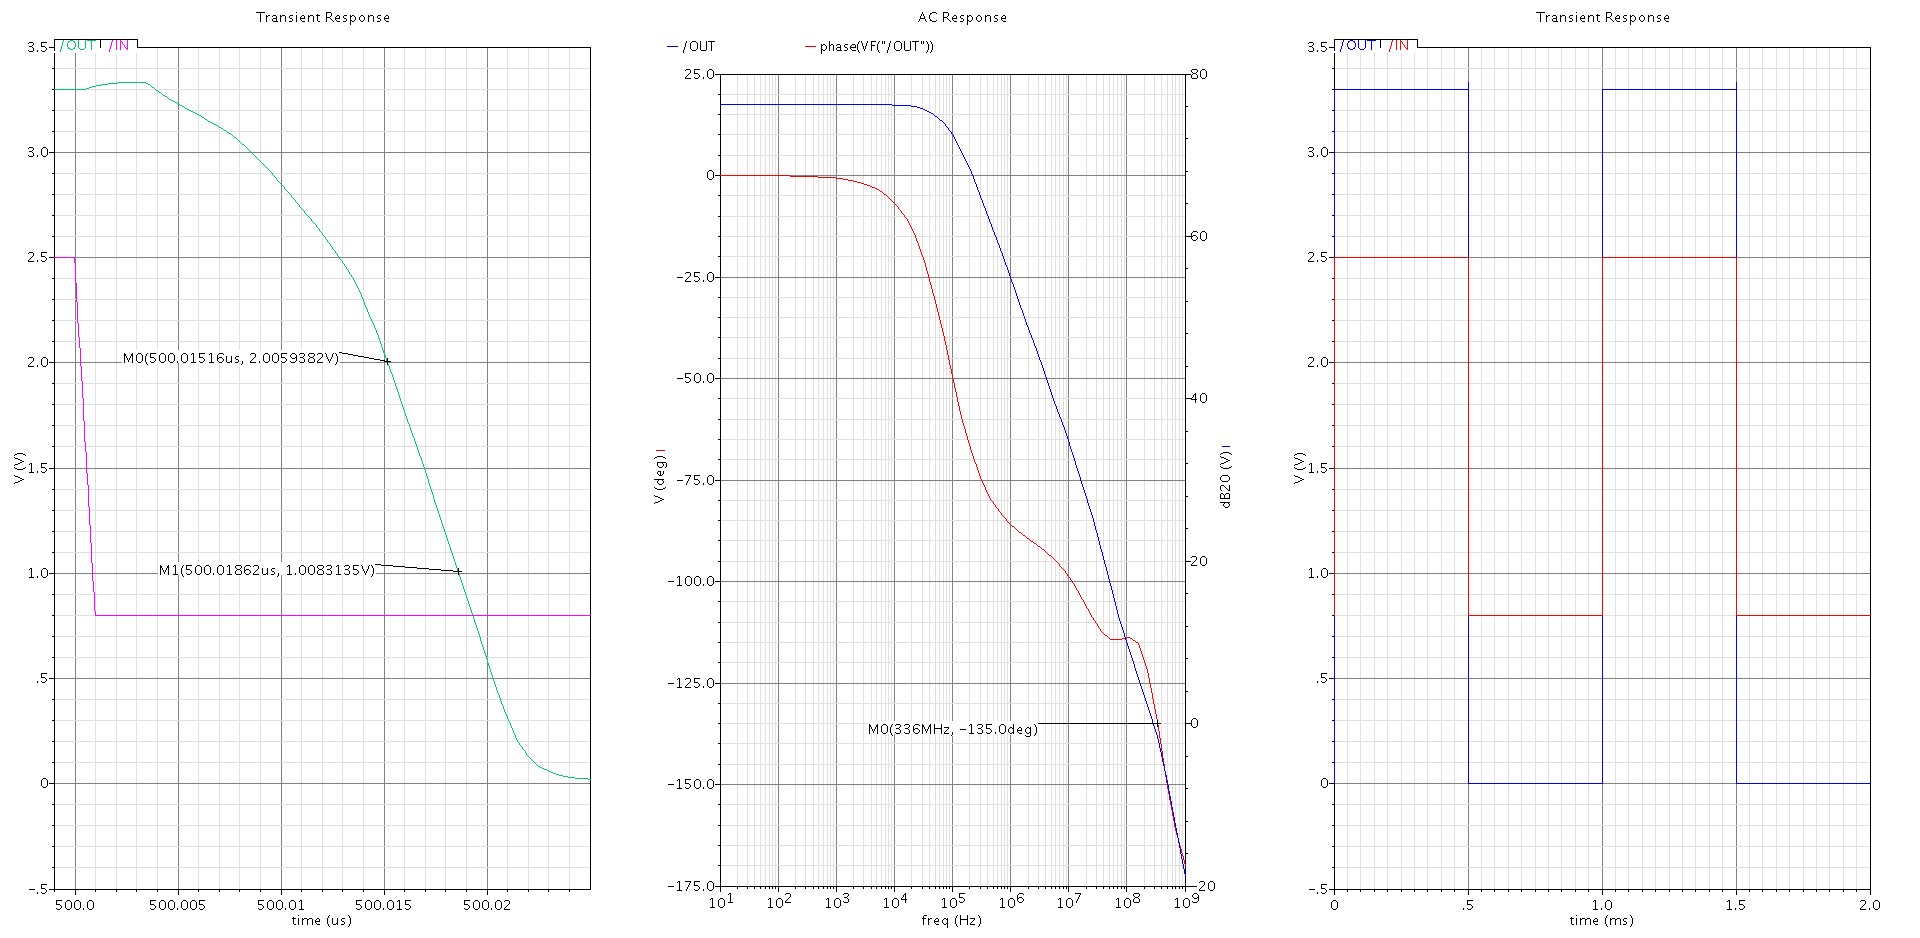
\includegraphics[keepaspectratio=true, scale=0.25]{exps/SIngle_Run}
	\vspace{-0.5em}
	\caption{Simulações efectuadas com o circuito final do \textit{middle target}.} 
	\vspace{-0.8em}
\end{figure} 

Relativamente às especificações que se pretende apresenta-se de seguida uma tabela com um resumo.

\begin{table}[H]
	\centering
	\caption{Especificações obtidas com o circuito final do \textit{middle target}.}
	\vspace{-1.5mm}
	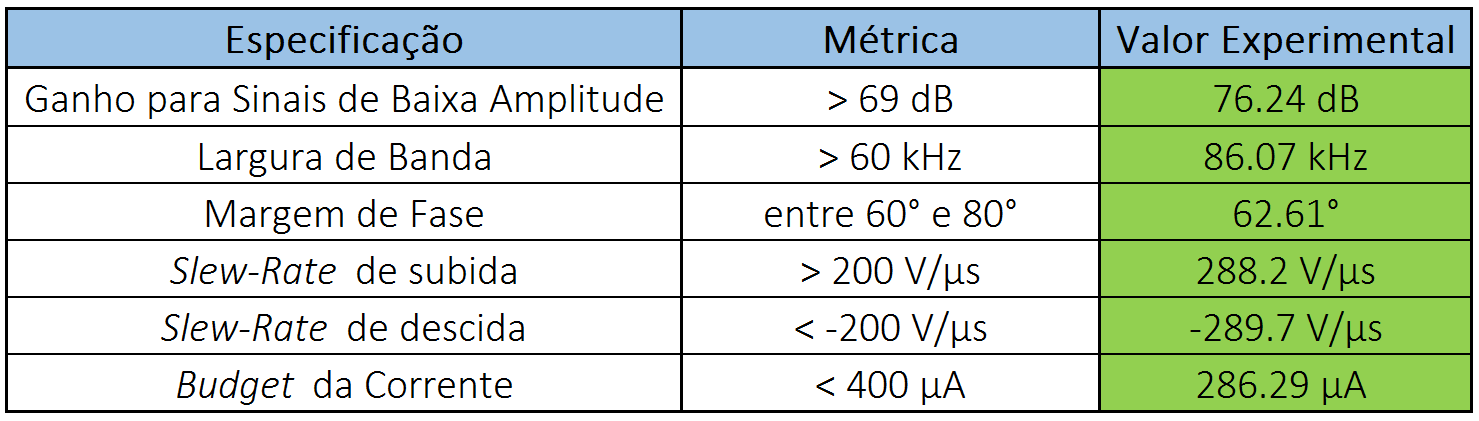
\includegraphics[keepaspectratio=true, scale=0.35]{teoricas/specsfinal}
\end{table}

\subsection{Demonstração de resultados} 

Nesta secção apresenta-se os resultados do dimensionamento do relatório intermédio e do novo dimensionamento anteriormente referido, para simulações de Monte Carlo e de \textit{corners}.

\subsubsection{Resultados do dimensionamento inicial} 

\begin{figure}[H]
	\centering
	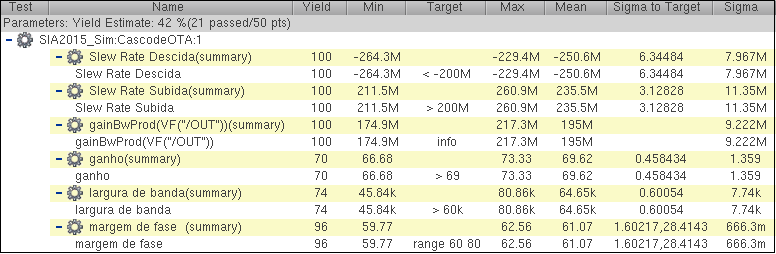
\includegraphics[keepaspectratio=true, scale=0.65]{exps/MonteCarlo_50pt_Antigo}
	\vspace{-0.5em}
	\caption{Simulação de Monte Carlo para 50 pontos.}
	\vspace{-0.8em}
\end{figure} 

\begin{figure}[H]
	\centering
	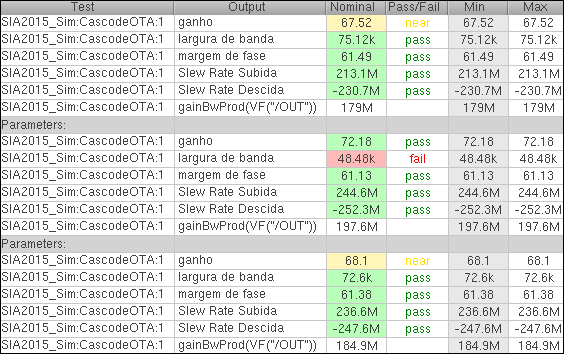
\includegraphics[keepaspectratio=true, scale=0.65]{exps/MonteCarlo_3pt_Antigo}
	\vspace{-0.5em}
	\caption{Resultados obtidos para as 3 primeiras simulações de Monte Carlo.}
	\vspace{-0.8em}
\end{figure} 

\begin{figure}[H]
	\centering
	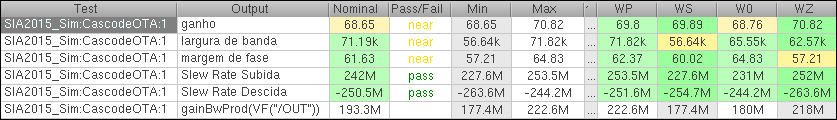
\includegraphics[keepaspectratio=true, scale=0.65]{exps/Corners_Antigo}
	\vspace{-0.5em}
	\caption{Simulação por \textit{corners}.}
	\vspace{-0.8em}
\end{figure} 

Tal como se pode observar das tabelas de resultados, antes das correções obtinha-se um \textit{yield} de 42\%, ou seja em cada quatro \textit{batches} pelo menos dois não seriam utilizáveis. Estas falhas eram maioritariamente devidas ao ganho e à largura de banda, pelo que, tal como se referiu anteriormente, foi especialmente aí que incidiram as correcções feitas. Tem-se também uma falha mínima na margem de fase levando a um \textit{yield} de 92\% que se poderia considerar aceitável. Verifica-se também que a simulação por \textit{corners} não apresenta os resultados desejados, sendo que, novamente, o ganho e a largura de banda apresentam os piores resultados, com a margem de fase a também ter falhas.

\subsubsection{Resultados do dimensionamento corrigido} 

\begin{figure}[H]
	\centering
	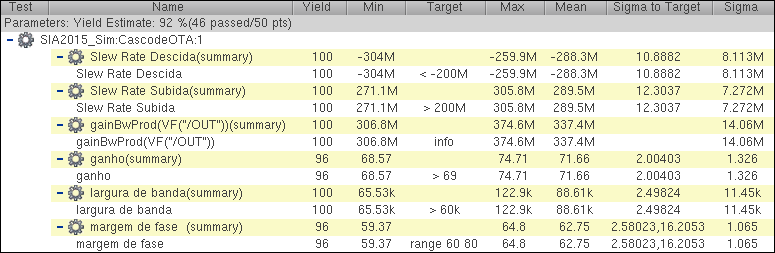
\includegraphics[keepaspectratio=true, scale=0.65]{exps/MonteCarlo_50pt_Novo}
	\vspace{-0.5em}
	\caption{Simulação de Monte Carlo para 50 pontos.}
	\vspace{-0.8em}
\end{figure} 

\begin{figure}[H]
	\centering
	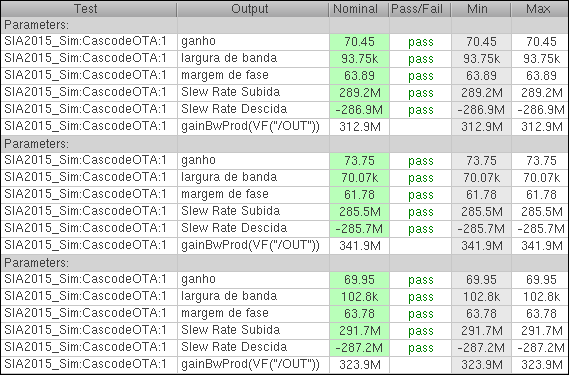
\includegraphics[keepaspectratio=true, scale=0.65]{exps/MonteCarlo_3pt_Novo}
	\vspace{-0.5em}
	\caption{Resultados obtidos para as 3 primeiras simulações de Monte Carlo.}
	\vspace{-0.8em}
\end{figure} 

\begin{figure}[H]
	\centering
	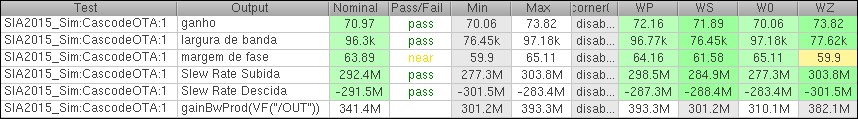
\includegraphics[keepaspectratio=true, scale=0.65]{exps/Corners_Novo_semDiv}
	\vspace{-0.5em}
	\caption{Simulação por \textit{corners}.}
	\vspace{-0.8em}
\end{figure} 

Após as correções os resultados são muito mais positivos, estando dentro dos requisitos do \textit{target}. O \textit{yield} final é de 96\% para 50 \textit{runs}, que se considera um resultado bastante aceitável. Considerou-se um valor de ganho de 69 dB, ou seja, inferior ao do \textit{target}. Esta consideração é permitida pois obteve-se um produto ganho largura de banda superior ao do \textit{target} nos casos em que não se obteve os 70 dB desejados pelo que, ao aplicar realimentação, se pode aumentar o ganho à custa de largura de banda, ficando-se dentro dos parâmetros desejados.

Na simulação por \textit{corners} obteve-se também resultados aceitáveis, sendo a única falha na margem de fase, com um erro de cerca de 1\%. 

\section{Projecção do \textit{layout}}

\subsection{Multiplicidade e \textit{fingers}}

Para projectar o \textit{layout} do circuito da Figura \ref{fig:finalint} optou-se por dividir os transístores de grandes dimensões com recurso a duas técnicas - multiplicidade e \textit{fingers}. A técnica de \textit{fingers} corresponde a um arranjo específico do transístor com $n$ \textit{gate fingers} em que as difusões da \textit{source} e do \textit{drain} são partilhadas. Se se tiver $n$ \textit{fingers} haverá então $n+1$ difusões. A multiplicidade é quando se faz uma ligação em paralelo de múltiplos dispositivos MOS, sendo que o agregado deles corresponde a um só transístor. Observa-se também que utilizar \textit{fingers} reduz a capacidade do transístor, aproximando-a da capacidade linear, sendo especialmente importante nos casos que afectem a largura de banda e margem de fase. 

Do ponto de vista da definição correspondem ao mesmo, mas são de facto duas maneiras diferentes de pensar na paralelização de transístores. Com o recurso a \textit{fingers} tem-se uma única célula com o transístor completo com todos os \textit{fingers}, útil para quando se quer uma célula mais compacta, enquanto na multiplicidade tem-se tantos transístores quanto a multiplicidade indicar. De facto, é possível conjugar as duas técnicas, ou seja, cada dispositivo MOS da multiplicidade pode ser feito com vários \textit{fingers}.

Para o trabalho em causa optou-se por usar as duas técnicas teoricamente idênticas para adquirir mais experiência e para verificar as diferenças que têm ao nível de implementação prática no Cadence.

Estas práticas são aplicadas também de forma a evitar  efeitos nocivos de \textit{mismatches}, ou seja da vulnerabilidade aos gradientes de parâmetro. Ao minimizar a área efectiva dos circuitos protege-se assim o dispositivo destes efeitos.

Assim sendo, deu-se especial atenção aos pares de transístores em que se considerou que existe uma maior sensibilidade a \textit{mismatches} - pares M\textsubscript{1}/M\textsubscript{2}, M\textsubscript{7}/M\textsubscript{8}, M\textsubscript{9}/M\textsubscript{10} e M\textsubscript{11\textsubscript{1}}/M\textsubscript{11\textsubscript{2}}. 

Começou-se, em primeira instância, por aplicar multiplicidade, tentando aproximar ao máximo os tamanhos dos pares que estão ligados entre si, seguido de uma redução geral dos transístores de todo o circuito. 

Em adição à multiplicidade optou-se por usar também a técnica \textit{fingers} no par M\textsubscript{7}/M\textsubscript{8} pois este par, tal como já foi mencionado, tem grande influência na largura de banda e margem de fase. Já no par M\textsubscript{5}/M\textsubscript{6} aplicou-se apenas a técnica \textit{fingers} ficando-se assim com tamanhos da mesma ordem em ambos os pares para além de uma forma compacta facilitando as tarefas de escolher uma disposição para os transístores e efectuar as ligações internas.

Como o rácio de espelhamento é muito sensível a diferenças nos parâmetros do espelho de corrente, ou seja, a \textit{mismatches} nos pares de transístores M\textsubscript{11\textsubscript{1}}/M\textsubscript{11\textsubscript{2}}, foi aplicada multiplicidade no transístor M\textsubscript{11\textsubscript{2}} de forma a que tivesse o mesmo tamanho que o transístor M\textsubscript{11\textsubscript{1}}. Desta maneira o par é afectado de igual forma pelos gradientes de parâmetros. Após a aplicação de multiplicidade nestes dois transístores foi necessário aumentar o valor da corrente \textit{Ibias} para 13 $\mu$A de forma a que se obtivesse o espelhamente correcto para 100 $\mu$A.

Para o par M\textsubscript{9}/M\textsubscript{10}, como são transístores NMOS, optou-se por colocar num grupo de apenas transístores NMOS, como será explicado à frente. Para este par apenas houve necessidade de reduzir os seus tamanhos através de multiplicidade para valores menos sensíveis a \textit{mismatches}.

Para os restantes transístores cuja sensibilidade a variação de parâmetros não é tão importante quanto nos pares supramencionados usou-se multiplicidade de forma a obter-se as dimensões desejadas e também que facilitassem as estruturas do \textit{layout}.

Assim, na tabela seguinte encontra-se uma descrição de como são constituídos os vários transístores do circuito.

\begin{table}[H]
	\centering
	\caption{Dimensões e características dos transístores do amplificador.}
	\vspace{-1.5mm}
	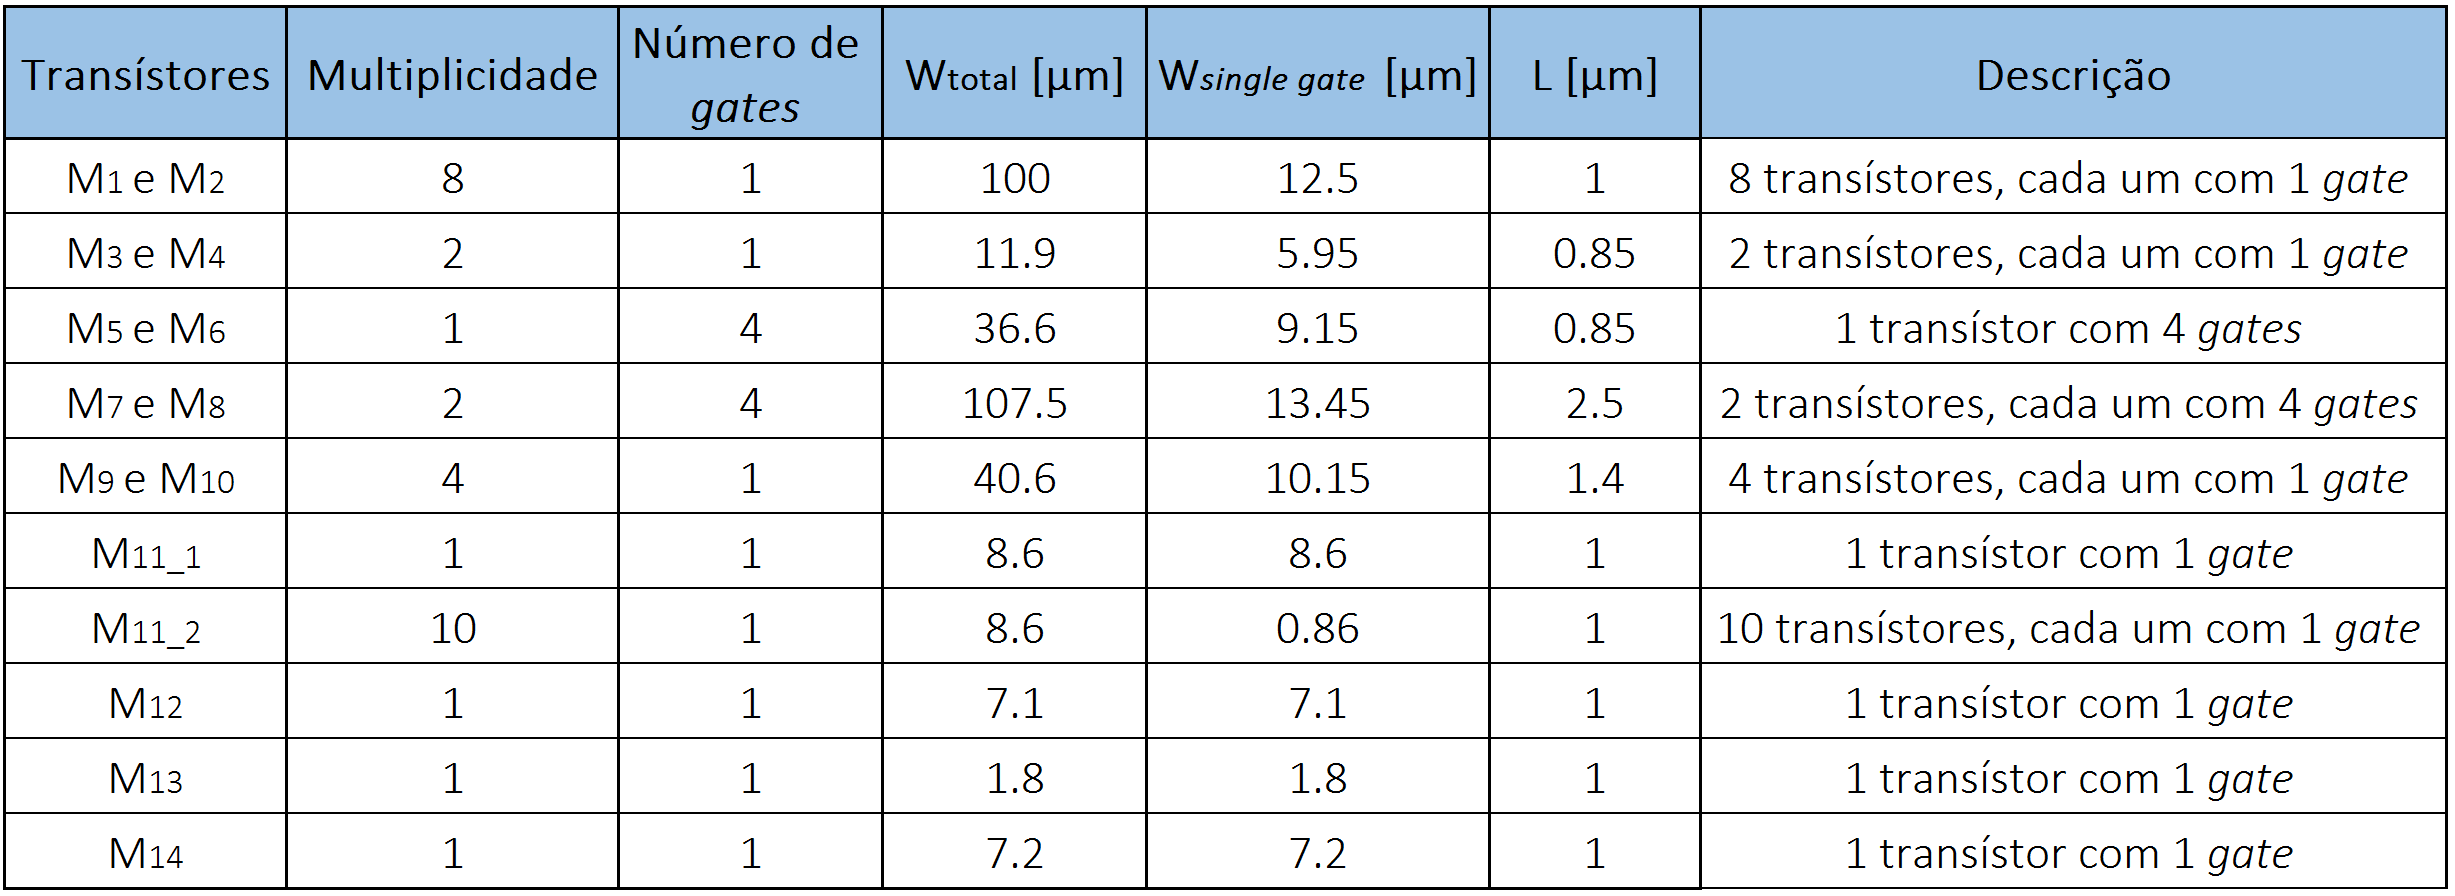
\includegraphics[keepaspectratio=true, scale=0.30]{teoricas/dimensoes2}
\end{table}

Na próxima figura apresenta-se o circuito após a divisão dos transístores com recurso a multiplicidade e \textit{fingers}.

\begin{figure}[H]
	\centering
	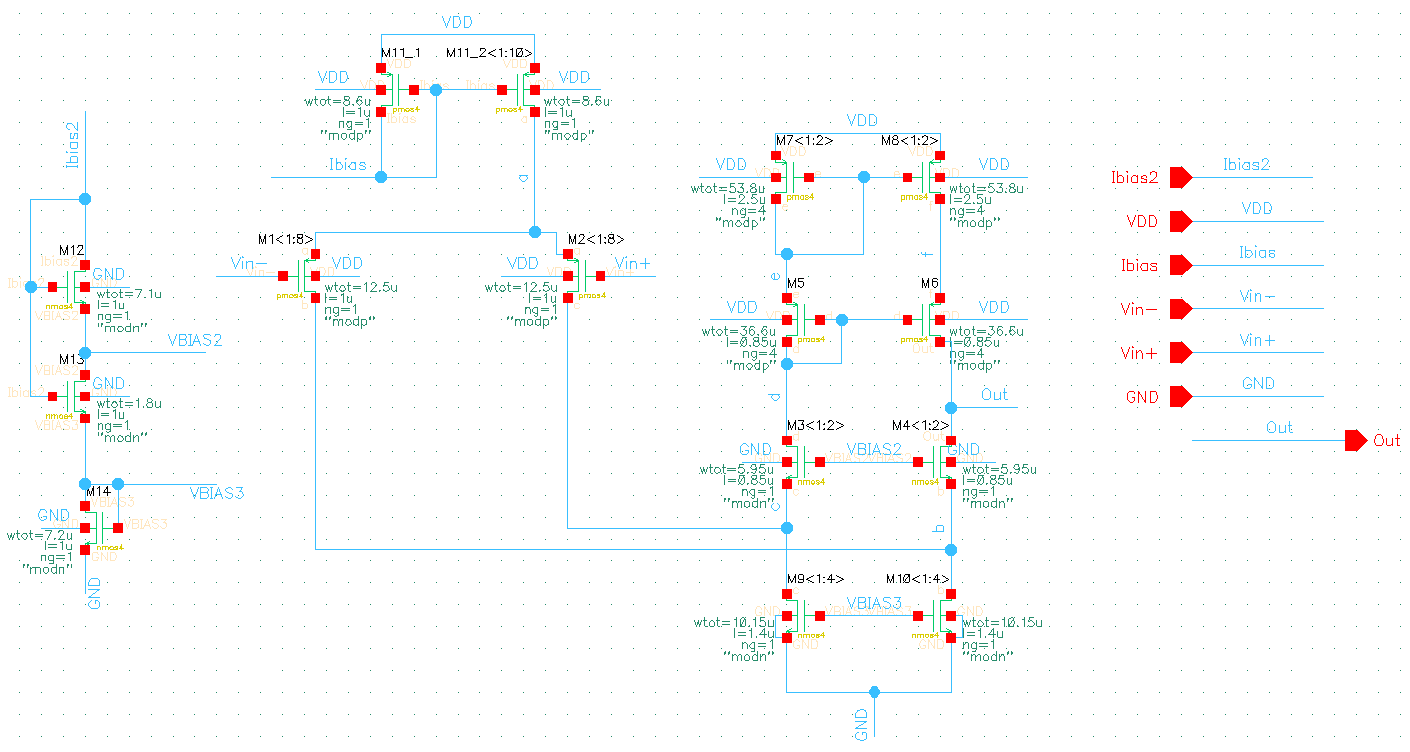
\includegraphics[keepaspectratio=true, scale=0.55]{exps/schematicdiv}
	\vspace{-0.5em}
	\caption{\textit{Schematic} do circuito para projecção do \textit{layout}.}
	\vspace{-0.8em}
\end{figure} 

Após realizar as alterações comentadas anteriormente realizou-se novamente uma simulação Monte Carlo de forma a observar os seus efeitos. Apresenta-se assim o obtido na figura seguinte.

\begin{figure}[H]
	\centering
	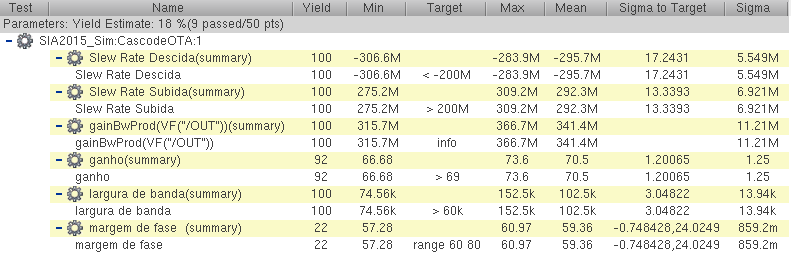
\includegraphics[keepaspectratio=true, scale=0.65]{exps/MonteCarlo_50pt_Novo_Sin}
	\vspace{-0.5em}
	\caption{Simulação Monte Carlo para 50 pontos após aplicar técnicas de multiplicidade e \textit{fingers}.}
	\vspace{-0.8em}
\end{figure} 

\begin{figure}[H]
	\centering
	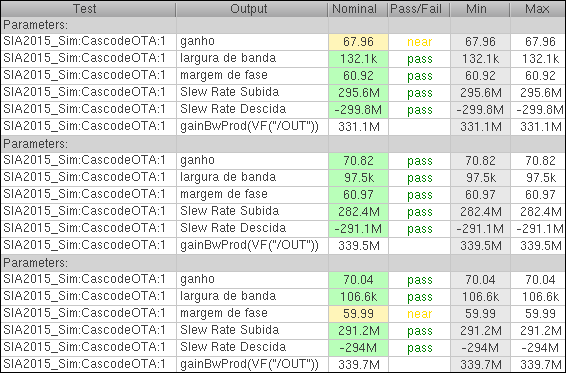
\includegraphics[keepaspectratio=true, scale=0.65]{exps/MonteCarlo_3pt_Novo_Sim}
	\vspace{-0.5em}
	\caption{Resultados obtidos para as 3 primeiras simulações de Monte Carlo após aplicar técnicas de multiplicidade e \textit{fingers}.}
	\vspace{-0.8em}
\end{figure} 

\begin{figure}[H]
	\centering
	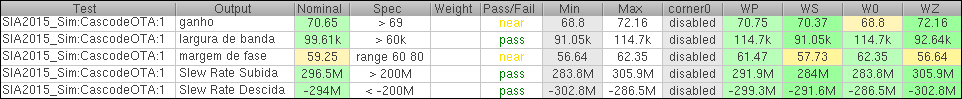
\includegraphics[keepaspectratio=true, scale=0.65]{exps/Corners_Novo_Sim}
	\vspace{-0.5em}
	\caption{Simulação por \textit{corners} após aplicar técnicas de multiplicidade e \textit{fingers}.}
	\vspace{-0.8em}
\end{figure}

Pode assim observar-se uma grande redução no \textit{yield}, tendo-se obtido 18\%. Isto é devido em grande parte à margem de fase, sendo que existe ainda uma ligeira descida nos resultados do ganho, mas que ainda assim iria levar a \textit{yields} aceitáveis. Esta influência na margem de fase deve-se à multiplicidade que faz aumentar o número de capacidades parasitas e a resistividade, que aliado à fraca optimização do \textit{layout} produzido automaticamente pelo Cadence, leva aos resultados observados. Este problema será em grande parte resolvido com as práticas tomadas para realizar o \textit{layout} como se irá explicar nas secções seguintes, pois o intuito destas é especificamente colmatar estes efeitos indesejados.

Em relação à simulação por \textit{corners} observa-se o mesmo tipo de resultados acima mencionados, sendo que os piores pertencem à margem de fase, pelo que este problema será em grande parte resolvido também pelas práticas correctas de layout que serão adoptadas.

\subsection{Disposição dos transístores}

Depois de se definir como estão estruturados os vários transístores é importante definir como se encontram dispostos no \textit{layout}. A topologia básica que foi utilizada é a de \textit{common centroid}. Através desta técnica consegue-se garantir um melhor \textit{matching} entre dois transístores iguais e em que se pretende um comportamento semelhante. De facto, o \textit{common centroid} é utilizado para se garantir que, e.g., um amplificador diferencial tenha um sinal de modo comum próximo de 0 e, como tal, um CMRR maior.

Para o circuito em causa foram definidos 4 blocos principais sobre os quais se definiu uma estrutura \textit{common centroid}:

\vspace{-2mm}

\begin{itemize}
	\item espelho de corrente básico que é polarizado em corrente com $I_{BIAS}$ (equivalente ao Bloco 1 da Figura 1) - estrutura \textit{common centroid} \#1;
	\vspace{-2mm}
	\item transístores do par diferencial (Bloco 2 da Figura 1) - estrutura \textit{common centroid} \#2;
	\vspace{-2mm}
	\item espelho de corrente cascode básico do tipo PMOS (Bloco 3 da Figura 1) - estrutura \textit{common centroid} \#3;
	\vspace{-2mm}
	\item transístores do tipo NMOS - estrutura \textit{common centroid} \#4;.
\end{itemize}

A escolha destes blocos foi feita com base no \textit{mismatch}. É essencial que entre os transístores do par diferencial não haja diferenças de comportamento, pois se houver o circuito fica desequilibrado. Os dois espelhos de corrente existentes também não devem ter \textit{mismatch}, pois pretende-se um espelhamento correcto. Como os transistores NMOS eram os mais pequenos e como não necessitam de estar dentro de um poço optou-se por juntar todos em apenas um bloco de forma a facilitar também a obtenção de \textit{common centroid} como será falado à frente.

De seguida apresenta-se as várias estruturas \textit{common centroid} definidas:

\begin{figure}[H]
	\centering
	\subfloat[]{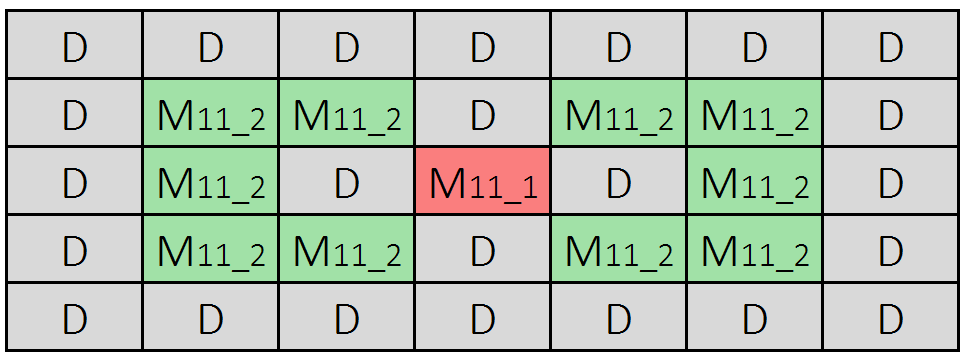
\includegraphics[keepaspectratio=true, scale=0.35]{teoricas/espelhodecorrente}}
	\hspace{8mm}
	\subfloat[]{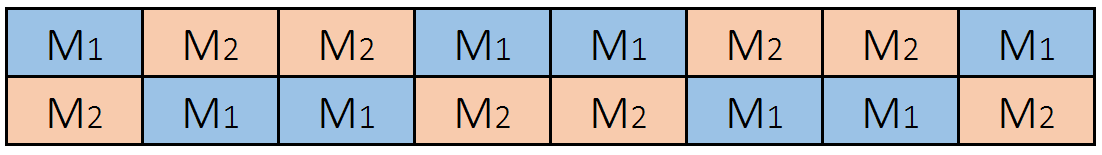
\includegraphics[keepaspectratio=true, scale=0.35]{teoricas/pardiferencial}}
	\linebreak
	\subfloat[]{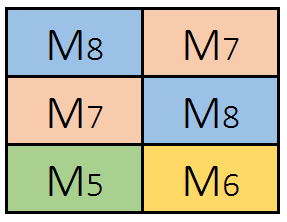
\includegraphics[keepaspectratio=true, scale=0.35]{teoricas/espelhodecorrenteamp}}
	\hspace{40mm}
	\subfloat[]{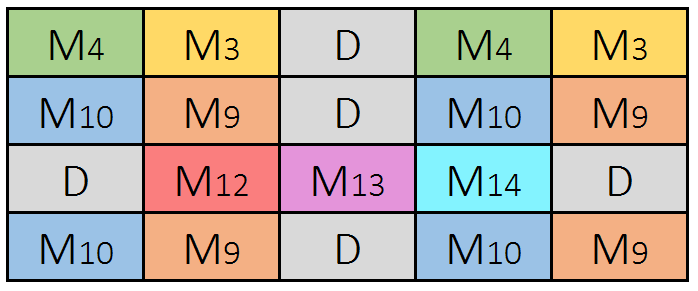
\includegraphics[keepaspectratio=true, scale=0.35]{teoricas/nmos}}
	\vspace{-0.8em}
	\caption{Estrutura \textit{common centroid} \#1 (a), \#2 (b), \#3 (c) e \#4 (d).}
	\vspace{-0.8em}
	\label{fig:common centroid}
\end{figure}

Nas figuras anteriores verifica-se a existências de transístores representados pela letra D - transístores \textit{dummies}. Este tipo de transístores serve para se garantir que os restantes transístores têm a mesma vizinhança, ou seja, que à sua volta vêem o mesmo. Veja-se o seguinte exemplo em que se consideram dois transístores - 1 e 2. O transístor 1 está definido com uma multiplicidade de 1 e o transístor 2 com uma multiplicidade de 8. Na figura seguinte encontra-se um exemplo de estrutura \textit{common centroid} para esse caso. 

\begin{figure}[H]
	\centering
	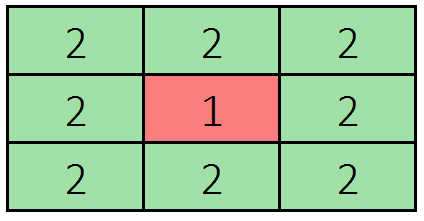
\includegraphics[keepaspectratio=true, scale=0.35]{teoricas/dummy1}
	\vspace{-0.5em}
	\caption{Exemplo de estrutura \textit{common centroid} com dois transístores.}
	\vspace{-0.8em}
\end{figure} 

O transístor 1 tem como vizinhança 4 transístores - para cima, para baixo, para a esquerda e para a direita. No entanto, qualquer transístor 2 tem uma ``falha'' naquilo que vê, pois não tem ``vizinhos'' nalgumas direcções. Assim, para se resolver este problema colocam-se transístores \textit{dummies} nos sítios onde há ``falhas''.

\begin{figure}[H]
	\centering
	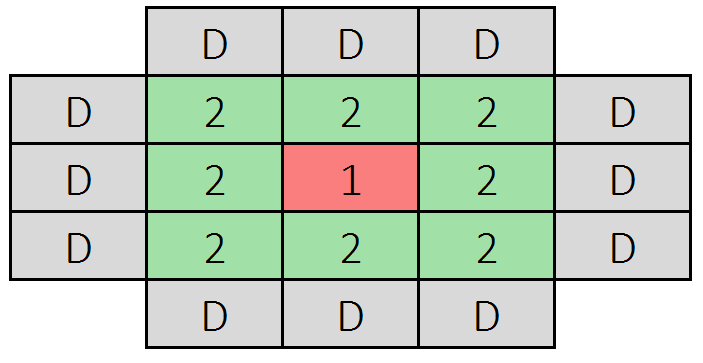
\includegraphics[keepaspectratio=true, scale=0.35]{teoricas/dummy2}
	\vspace{-0.5em}
	\caption{Exemplo de estrutura \textit{common centroid} com dois transístores e também transístores \textit{dummies}.}
	\vspace{-0.8em}
\end{figure}

De facto, os transístores \textit{dummies} não necessitam de ter as mesmas dimensões que os restantes e o circuito da figura anterior pode ser definido da seguinte maneira.

\begin{figure}[H]
	\centering
	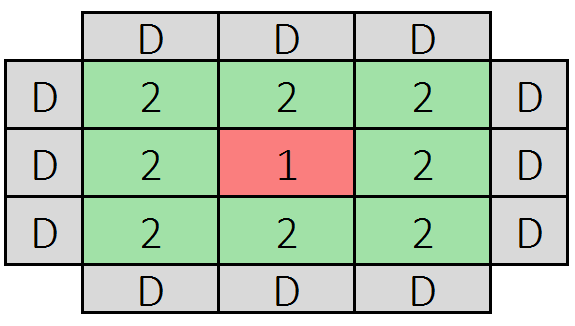
\includegraphics[keepaspectratio=true, scale=0.35]{teoricas/dummy3}
	\vspace{-0.5em}
	\caption{Exemplo de estrutura \textit{common centroid} com dois transístores e também transístores \textit{dummies} de dimensões menores.}
	\vspace{-0.8em}
\end{figure}

Relembrando as estruturas da Figura \ref{fig:common centroid}, verifica-se que a estruturas \#1 e \#4 têm \textit{dummies}.

Na caso da estrutura \#1, tinha-se à partida 11 transístores de dimensões iguais após a aplicação de multiplicidade. Como se quer garantir que todos os transístores observem as mesmas vizinhanças, minimizando o efeito de \textit{mismatches}, fez-se uso de \textit{dummies} para ocupar as lacunas que iriam, de outra forma, ficar vazias. O ponto de partida foi assim o transístor M\textsubscript{11\textsubscript{1}} em que não se aplicou multiplicidade rodeando-o dos 10 transístores que constituem M\textsubscript{11\textsubscript{2}}. Após isto observou-se que seria assim necessário 24 \textit{dummies}. Posto isto obtém-se uma estrutura rectangular de 5$\times$7 em que todos os M\textsubscript{11\textsubscript{2}}, assim como o transístor M\textsubscript{11\textsubscript{1}}, observam as mesmas vizinhanças.
		
Para a estrutura \#4 o procedimento foi similar. Tinha-se à partida os 3 transístores de polarização M\textsubscript{12}, M\textsubscript{13} e M\textsubscript{14} aos quais não foi aplicada nem multiplicidade nem \textit{fingers} pois já têm tamanhos bastante reduzidos. Para que se pudesse garantir que eles tinham as mesmas vizinhanças teriam que ser rodeados de \textit{dummies}. Como no entanto se tratam de transístores do tipo N e tinha sido decidido colocar todos os transístores deste tipo no mesmo bloco bastou adicionar-se os pares  M\textsubscript{3}/M\textsubscript{4} e  M\textsubscript{9}/M\textsubscript{10}, colocando-os de forma alternada obtendo-se o esquema da Figura \ref{fig:common centroid}(d). Como todos os transístores presentes neste bloco têm tamanhos muito díspares fica-se com uma estrutura final que apresenta algumas áreas vazias. Estes espaços vazios são no entanto necessários para garantir que todos os transístores observam as mesmas vizinhanças, ajudando assim a garantir o objectivo de reduzir os efeitos de \textit{mismatch}.

\subsection{Ligações internas dos blocos}

Uma vez definidos como estão estruturados os transístores e como estão dispostos efecutam-se as ligações internas dos 4 blocos da Figura \ref{fig:common centroid}.

Existem várias regras para construir um \textit{layout}, sendo que uma delas impõe um espaço mínimo para separar as diferentes máscaras. Para evitar isto, recorre-se a uma opção existente no Cadence que notifica o utilizador quando este não cumpre as margens mínimas. 

As ligações entre \textit{gates} de transístores que estejam próximos são feitas a partir da camada condutora \texttt{poly}. Porém, se os transístores estiverem afastados é preferível efectuar a ligação com recurso a \texttt{Metal1} e a contactos do tipo \texttt{P1\_C}, que efectuam a ligação entre \texttt{poly} e \texttt{Metal1}. Esta solução é preferível para esses casos pois a \texttt{poly} tem uma resistividade elevada e colocar demasiado dessa camada faz aumentar a resistividade geral do circuito. De facto, na tabela seguinte apresenta-se a resistividade das diversas máscaras existentes no fabrico e verifica-se que a \texttt{poly} (\texttt{poly1}) tem uma resistividade bem superior face a camadas como \texttt{Metal1} e \texttt{Metal2}. Verifica-se também que a resistividade de um contacto do tipo \texttt{P1\_C} é elevada, mas que compensa, uma vez que para efectuar uma ligação correcta entre duas \textit{gates} bastaria colocar no máximo 2 contactos.

\begin{table}[H]
	\centering
	\caption{Resistividade das diversas máscaras de fabrico (a) e resistividade dos diversos tipos de contactos (b).}
	\vspace{-1.5mm}
	\subfloat[]{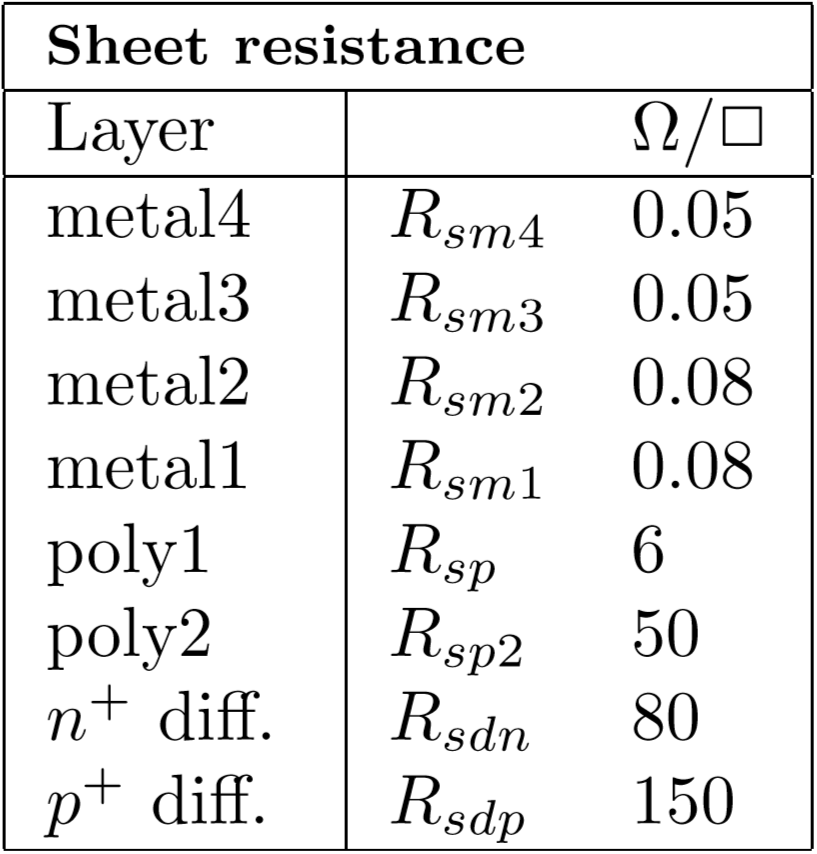
\includegraphics[keepaspectratio=true, scale=0.20]{teoricas/resistance}}
	\hspace{8mm}
	\subfloat[]{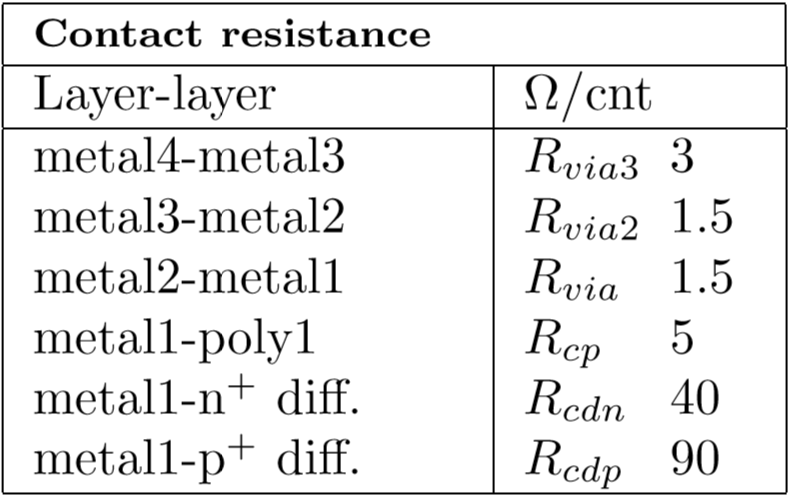
\includegraphics[keepaspectratio=true, scale=0.27]{teoricas/resistanceC}}
	\vspace{-0.8em}
\end{table}

Tomou-se a decisão de, sempre que possível, efectuar as ligações com \texttt{Metal1} na horizontal e com \texttt{Metal2} na vertical. Procura-se aplicar esta \textit{rule of thumb} sempre que possível, sendo que apenas não é cumprida quando se verifica que acaba por tornar mais difícil o \textit{design} do \textit{layout} ou que conduz a uma área maior porque é necessário ajustar o espaçamento entre transístores para acomodar uma ligação em \texttt{Metal1} ou \texttt{Metal2} consoante o caso.

Para ligar \texttt{Metal1} a \texttt{Metal2} é usada uma via. De referir que, optou-se também, sempre que possível, por colocar vias e contactos duplos, para que houvesse um de \textit{backup}. À semelhança do que se referiu anteriormente, isto é feito quando não dificulta o \textit{design} do \textit{layout}.

\subsubsection{Estrutura \textit{common centroid} \#1}

Relembrando a estrutura da Figura \ref{fig:common centroid}(a), a sua primeira implementação no Cadence foi feita da seguinte maneira:

\begin{figure}[H]
	\centering
	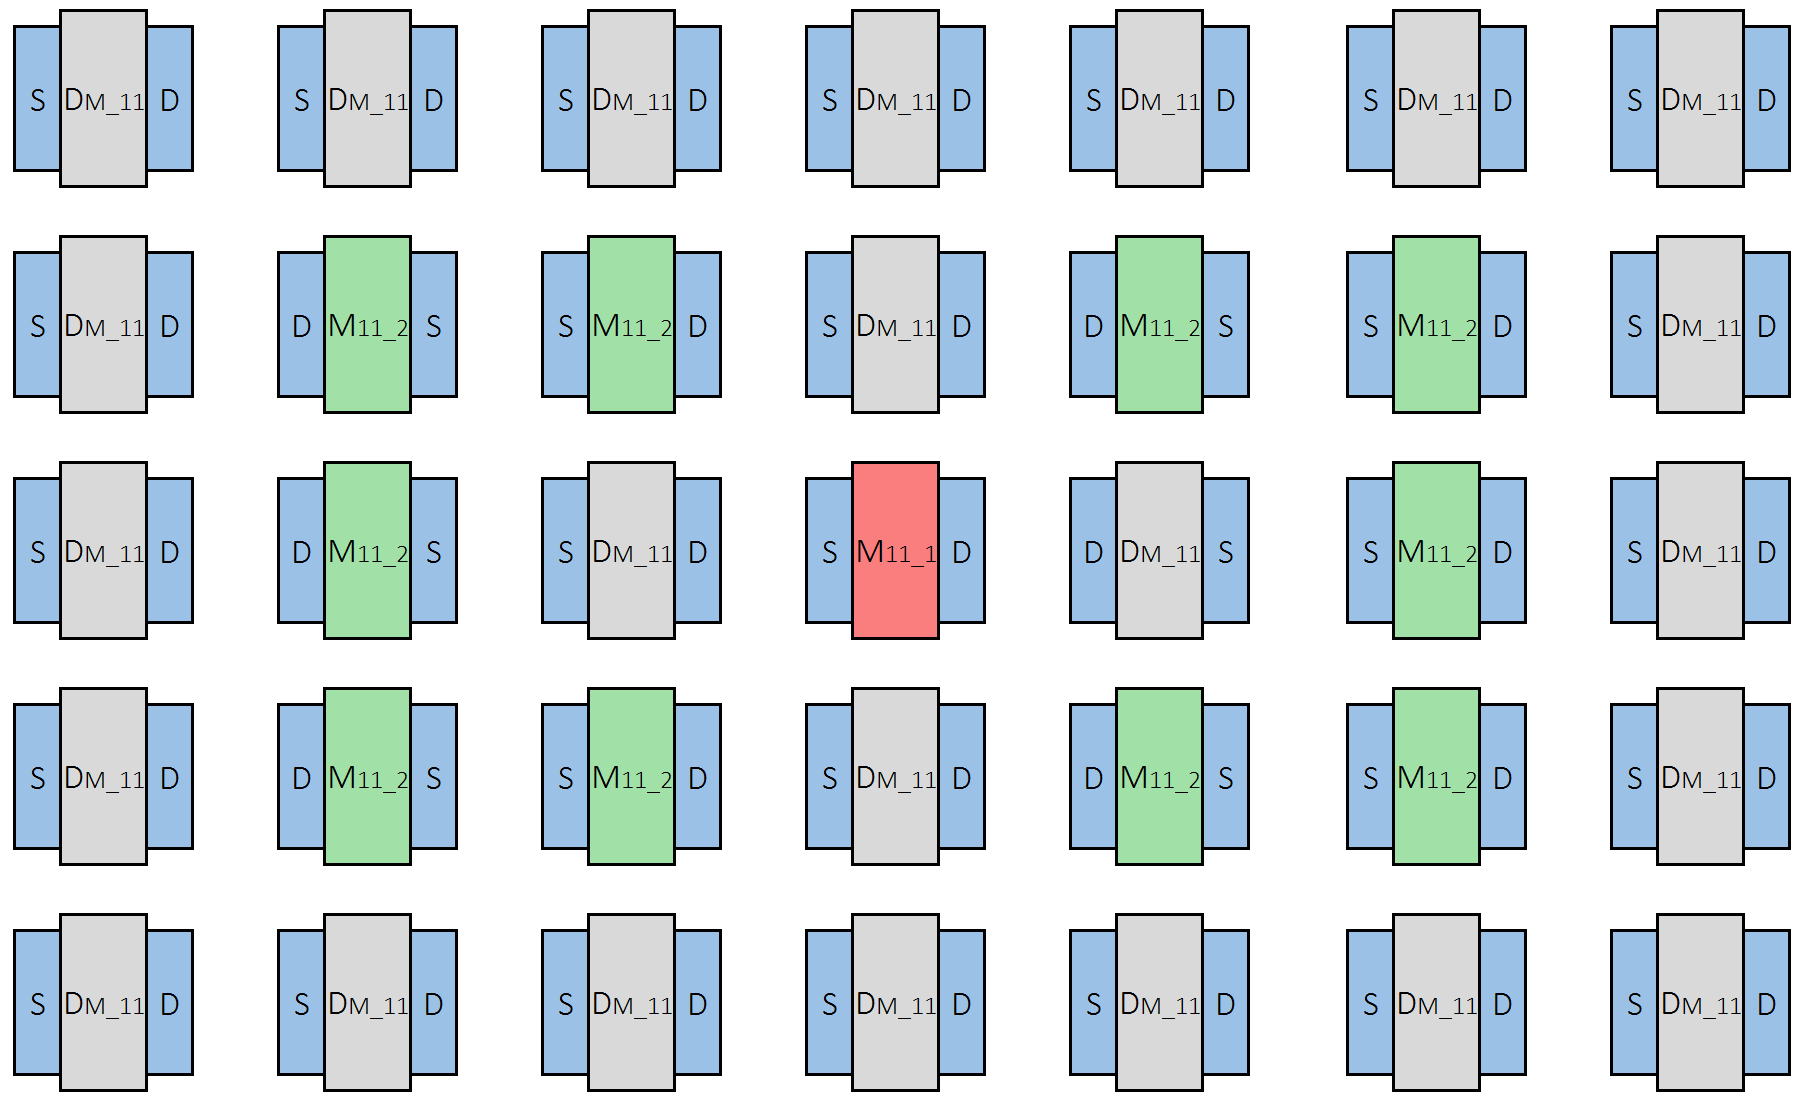
\includegraphics[keepaspectratio=true, scale=0.30]{teoricas/layout/cc1_1}
	\vspace{-0.5em}
	\caption{Esquema inicial do \textit{layout}.}
	\vspace{-0.8em} 
\end{figure}

Como se pode ver, da maneira como a estrutura \textit{common centroid} foi definida é possível sobrepor as difusões de \textit{source} dos transístores M\textsubscript{11\textsubscript{2}}, poupando assim área. Da mesma maneira, pode-se também sobrepor a \textit{source} do transístor M\textsubscript{11\textsubscript{2}} do meio com a \textit{source} do transístor \textit{dummy} que se encontra próximo do transístor M\textsubscript{11\textsubscript{1}}. Desta maneira, o circuito fica com a seguinte estrutura:

\begin{figure}[H]
	\centering
	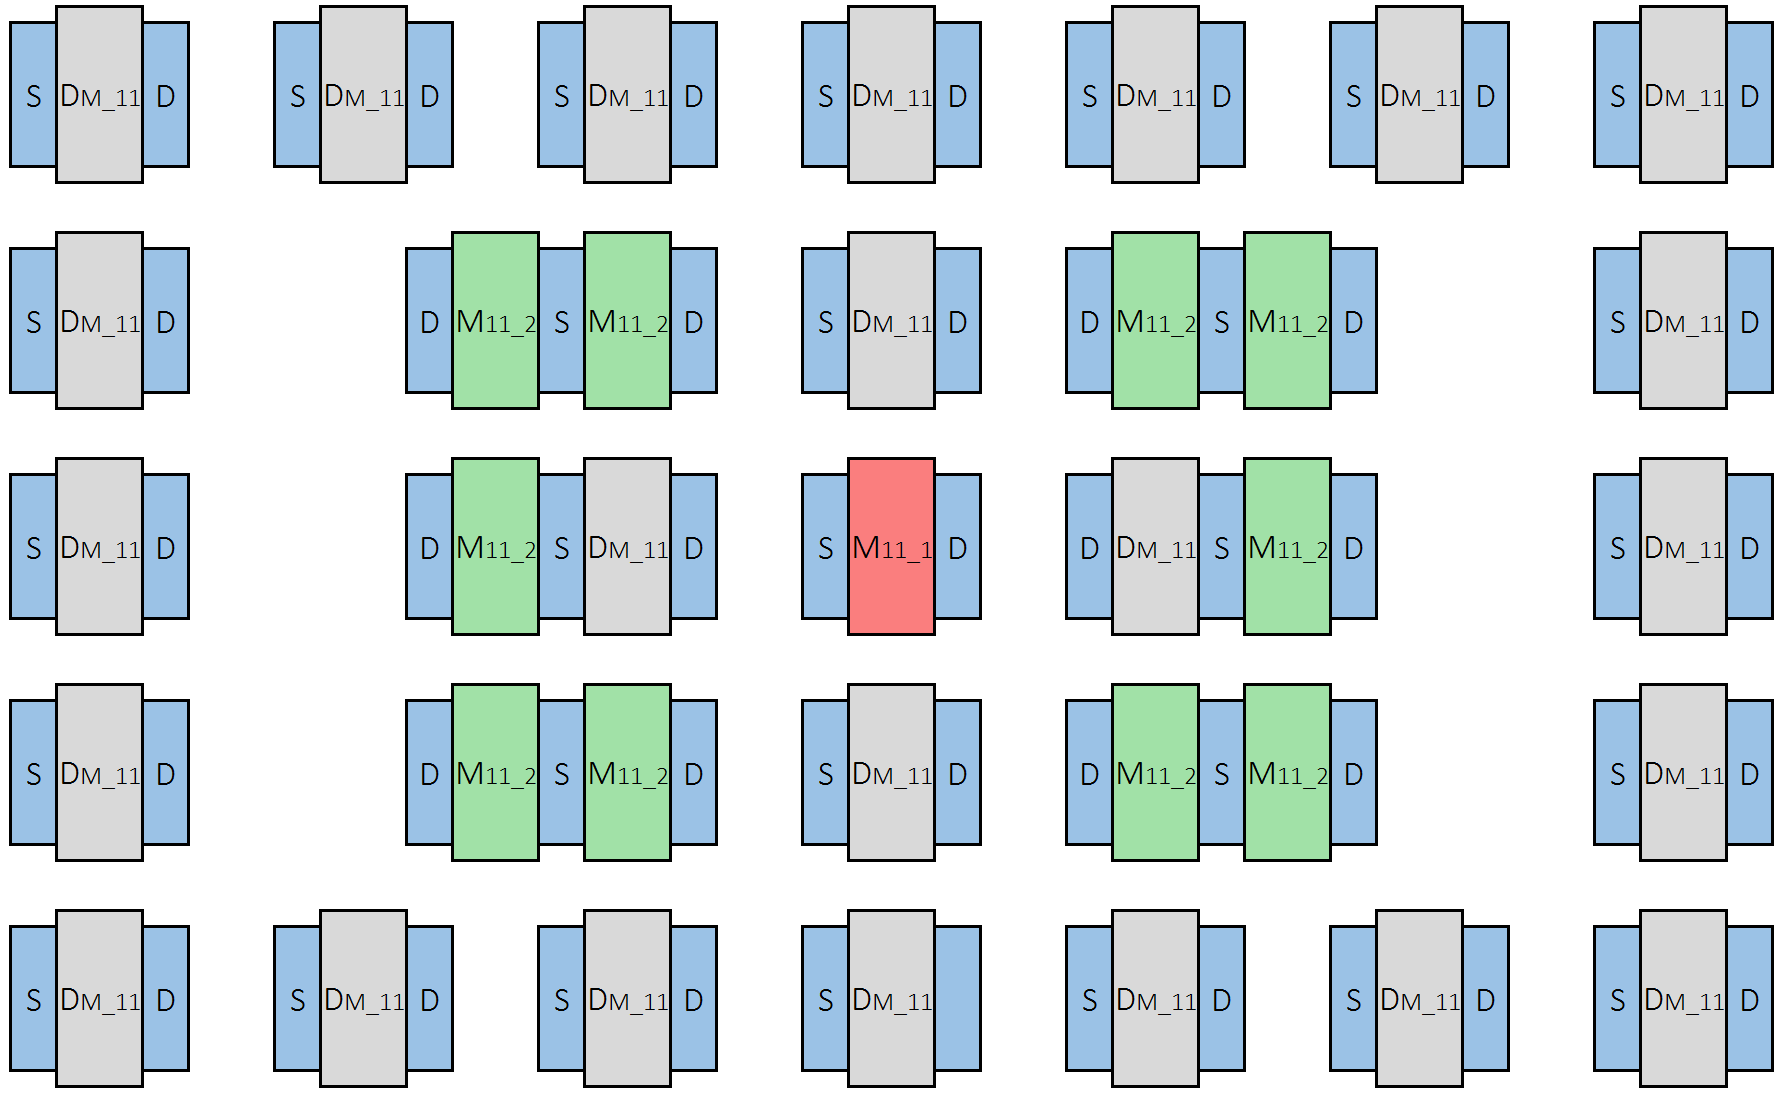
\includegraphics[keepaspectratio=true, scale=0.30]{teoricas/layout/cc1_2}
	\vspace{-0.5em}
	\caption{Estrutura resultante da agregação das difusões de alguns transístores.}
	\vspace{-0.8em} 
\end{figure}

No entanto, verifica-se que agora as vizinhanças dos transístores não estão de acordo com o pretendido, havendo ``buracos'' entre a estrutura rectangular de \textit{dummies} e a estrutura rectangular interior. Assim, optou-se por ajustar a estrutura exterior com \textit{dummies} de menores dimensões  e de modo a que a estrutura geral ficasse rectangular, apenas com o espaço necessário mínimo entre transístores que garante um correcto funcionamento do circuito. Outra razão para o interesse de reduzir as dimensão total do bloco irá ser evidenciada à frente, pois seria impossível polarizar todo o bloco recorrendo apenas a um \textit{guard ring}. O aspecto final é então como se segue.

\begin{figure}[H]
	\centering
	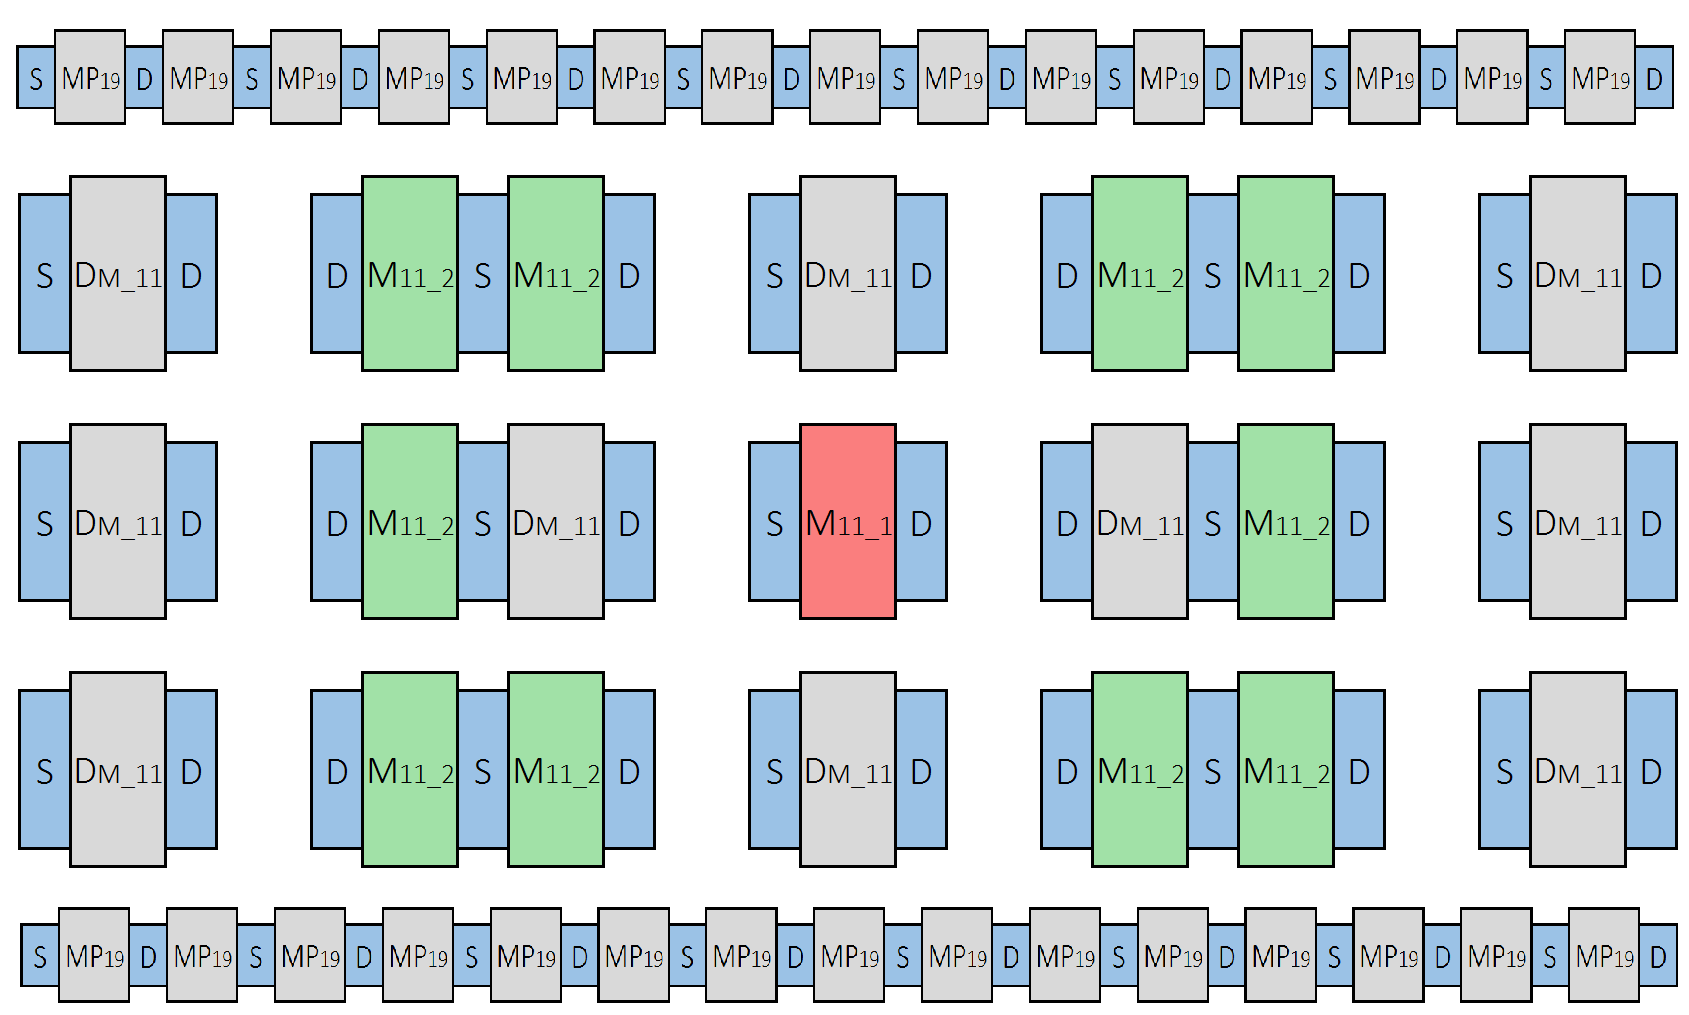
\includegraphics[keepaspectratio=true, scale=0.30]{teoricas/layout/cc1_3}
	\vspace{-0.5em}
	\caption{Estrutura resultante do \textit{layout} do espelho de corrente básico que é polarizado em corrente com $I_{BIAS}$.}
	\vspace{-0.8em} 
\end{figure} 

A implementação desta estrutura no Cadence é apresentada de seguida.

\begin{figure}[H]
	\centering
	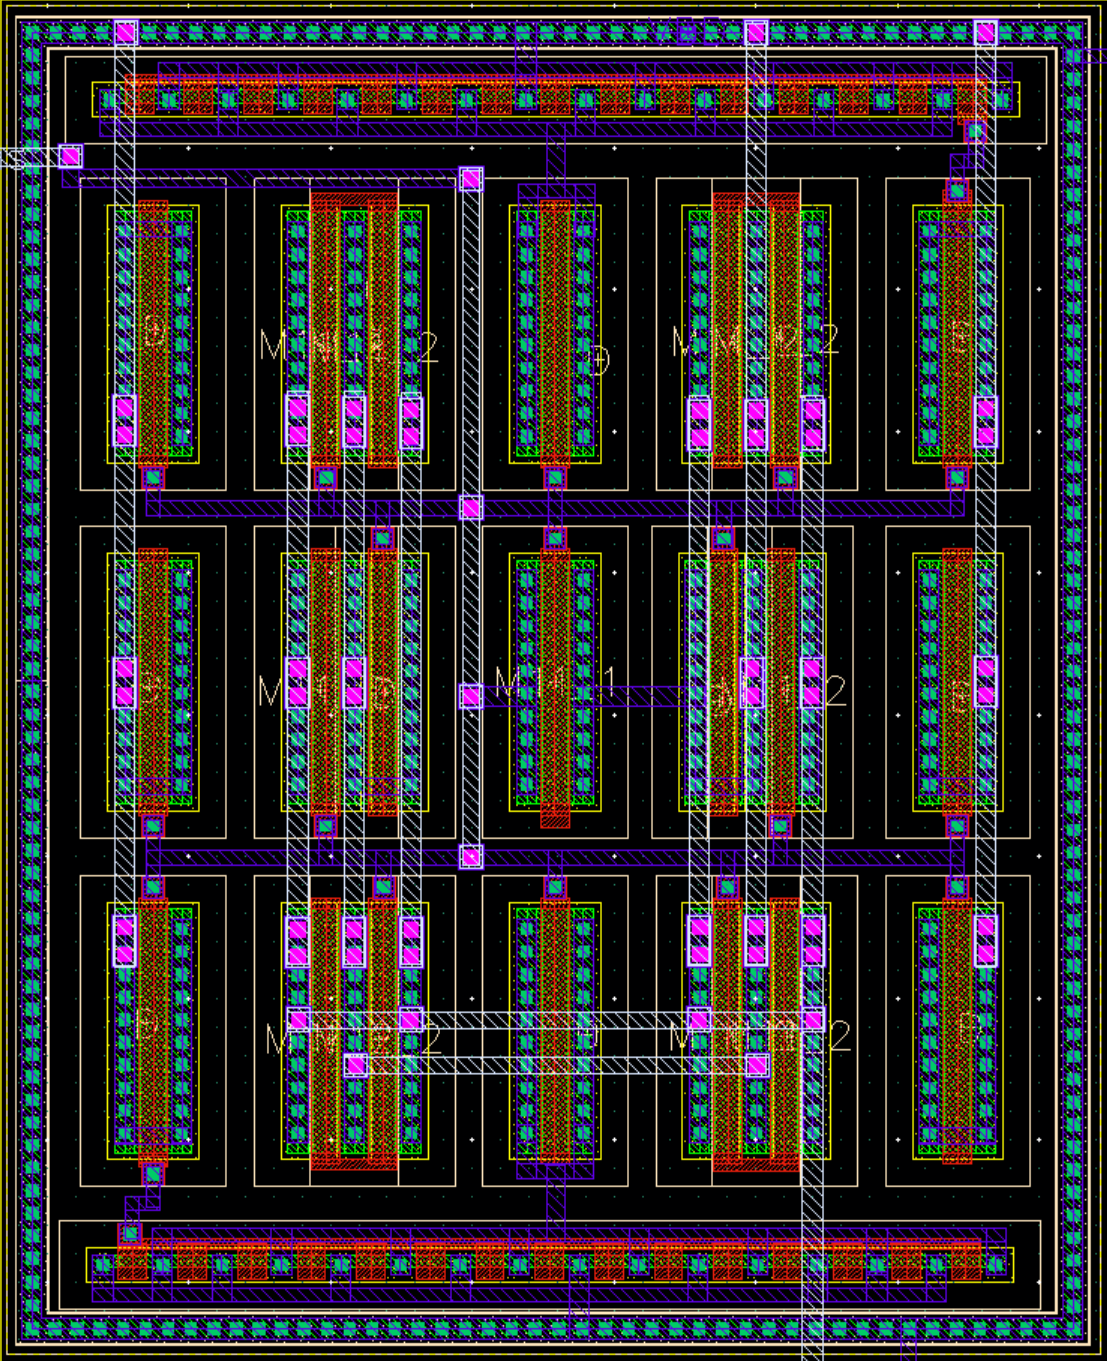
\includegraphics[keepaspectratio=true, scale=0.65]{exps/layout/espelhodecorrente}
	\vspace{-0.5em}
	\caption{\textit{Layout} da estrutura que corresponde ao espelho de corrente básico que é polarizado em corrente com $I_{BIAS}$.}
	\vspace{-0.8em}
\end{figure}

Como se pode ver, as \textit{gates} dos transístores \textit{dummy} foram ligadas a $I_{BIAS}$ e não a VDD, como seria esperado, para fazer curto-circuito aos \textit{dummies} do tipo P. A razão pela qual se faz isto é que, ao fazer estas ligações, cria-se um condensador entre $I_{BIAS}$ e VDD como se demonstra na figura seguinte.

\begin{figure}[H]
	\centering
	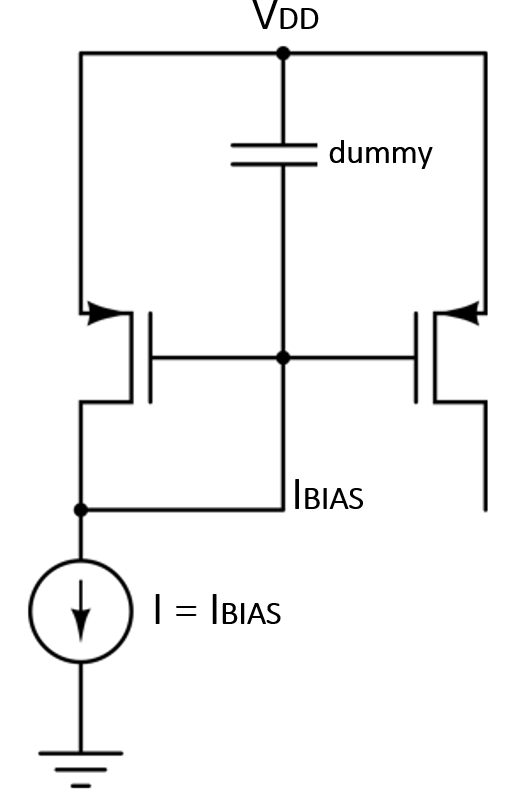
\includegraphics[keepaspectratio=true, scale=0.45]{teoricas/circuito_ibias}
	\vspace{-0.5em}
	\caption{Circuito que demonstra o efeito de ligar as \textit{gates} dos \textit{dummies} a $I_{BIAS}$.}
	\vspace{-0.8em}
\end{figure}

Desta forma protege-se o \textit{dummy} de variações na fonte de tensão que de outra forma iriam comprometer a integridade do transístor e como tal a do espelho de corrente, pois este condensador irá actuar como um filtro apenas aquando a ocorrência de variações.

Quando se extraiu o \textit{layout} do circuito verificou-se de facto a existência deste condensador, como se pode ver na figura seguinte. 

\begin{figure}[H]
	\centering
	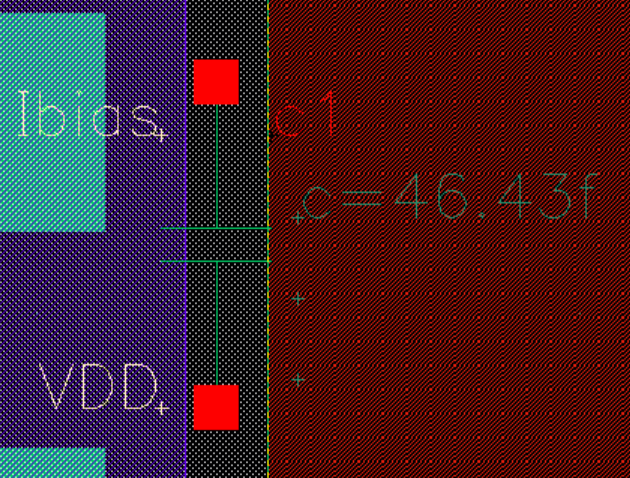
\includegraphics[keepaspectratio=true, scale=0.35]{exps/condensador1}
	\vspace{-0.5em}
	\caption{Condensador que surge entre $I_{BIAS}$ e VDD.}
	\vspace{-0.8em}
\end{figure}

Analisando a capacidade do condensador, 46.43 F, verifica-se que é um valor elevado, o que é representativo da influência dos \textit{dummies} no circuito, não sendo esta apenas uma capacidade parasita.

Como se pode ver, em torno dos transístores PMOS foi colocado um poço, ou seja, aplicou-se a máscara \texttt{NTUB}. Isso tem de ser feito porque no caso dos transístores PMOS, as difusões do tipo $p$+ não podem estar directamente ligadas ao substrato, uma vez que este é do tipo $p+$. Assim, é necessário criar um poço do tipo $n$ entre as difusões e o substrato.

É de referir que dentro do poço encontra-se um \textit{guard ring} do tipo \texttt{ndiff\_ntub}. Através deste é possível polarizar o substrato a VDD, colocando sobre o \textit{guard ring} o \textit{pin} correspondente tal como se observa na figura

\begin{figure}[H]
	\centering
	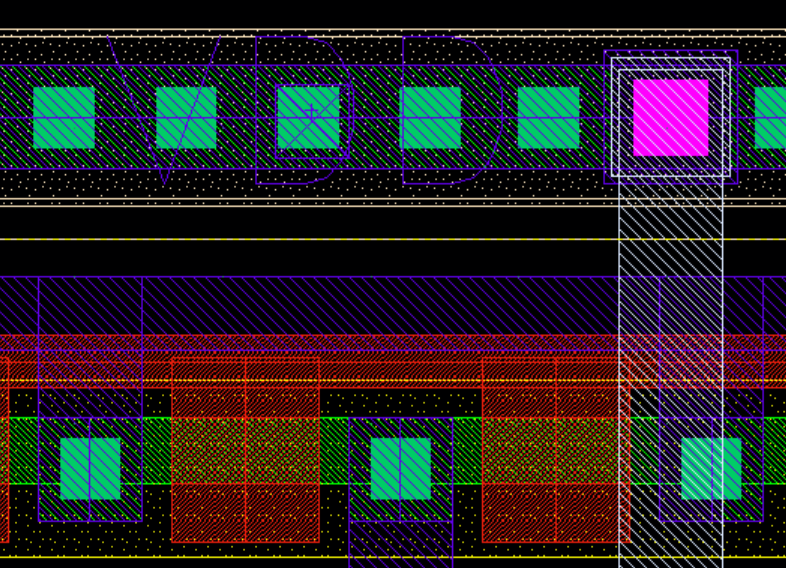
\includegraphics[keepaspectratio=true, scale=0.25]{exps/layout/pinVDD}
	\vspace{-0.5em}
	\caption{Colocação do \textit{pin} de VDD sobre o \textit{guard ring}.}
	\vspace{-0.8em}
\end{figure}

De forma a que o bloco esteja bem polarizado, todos os pontos deste deveriam estar a uma distância mínima de 20 $\mu$m. Isto seria impossível com as dimensões iniciais pelo que se realizou a redução tal como foi indicado anteriormente obtendo-se assim uma distância ao centro inferior a 17 $\mu$m ficando portanto correctamente polarizado.

O \textit{guard ring} tem também o intuito de proteger o circuito de correntes de dispersão e, desta maneira, o ruído do substrato encontra no \textit{guard ring} blindagem.

É de referir que nesta altura da projecção do \textit{layout} quando se efectuava um DRC e um LVS sobre o \textit{design} do circuito havia dois problemas principais - \textit{hot nwell} e mau \textit{match} entre os \textit{pins} do \textit{schematic} e do \textit{layout}. O problema de \textit{hot nwell} surge quando o substrato não está correctamente polarizado a VDD, que acontecia devido ao segundo erro mencionado. De forma a que se polarize correctamente o \textit{guard ring} o material do \textit{pin} e da \textit{label} devem assim ser de materiais complementares, ou seja, o \textit{pin} é do material \texttt{Metal1} \texttt{Pin} e a \textit{label} terá que ser do material \texttt{Pin} \texttt{Metal1}. Com isto ficam corrigidos ambos os erros.

\subsubsection{Estrutura \textit{common centroid} \#2}

Relembrando a estrutura da Figura \ref{fig:common centroid}(b), a sua primeira implementação no Cadence foi feita da seguinte maneira:

\begin{figure}[H]
	\centering
	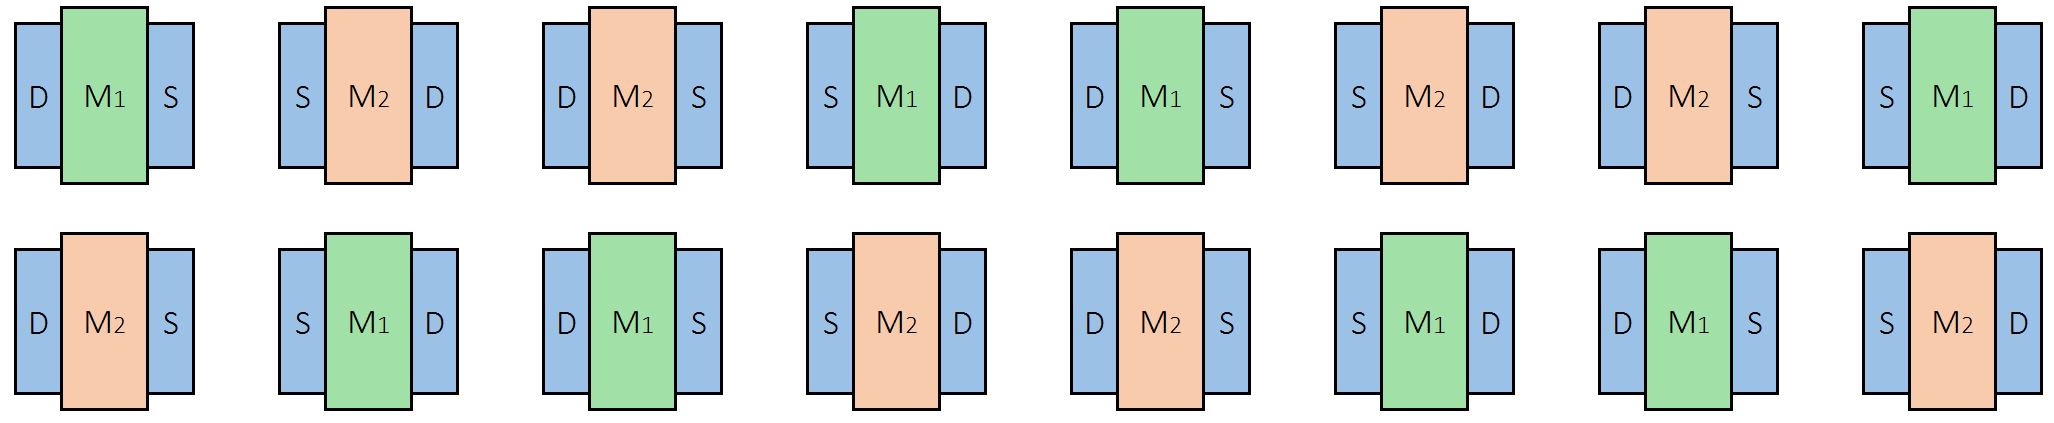
\includegraphics[keepaspectratio=true, scale=0.30]{teoricas/layout/cc2_1}
	\vspace{-0.5em}
	\caption{Esquema inicial do \textit{layout}.}
	\vspace{-0.8em} 
\end{figure}

É de referir que, sabendo que as \textit{sources} de M\textsubscript{1} e M\textsubscript{2} estão ligadas ao mesmo ponto (saída do espelho de corrente que polariza o circuito), pode-se sobrepor as suas difusões, ficando assim o \textit{layout} com a seguinte estrutura.

\begin{figure}[H]
	\centering
	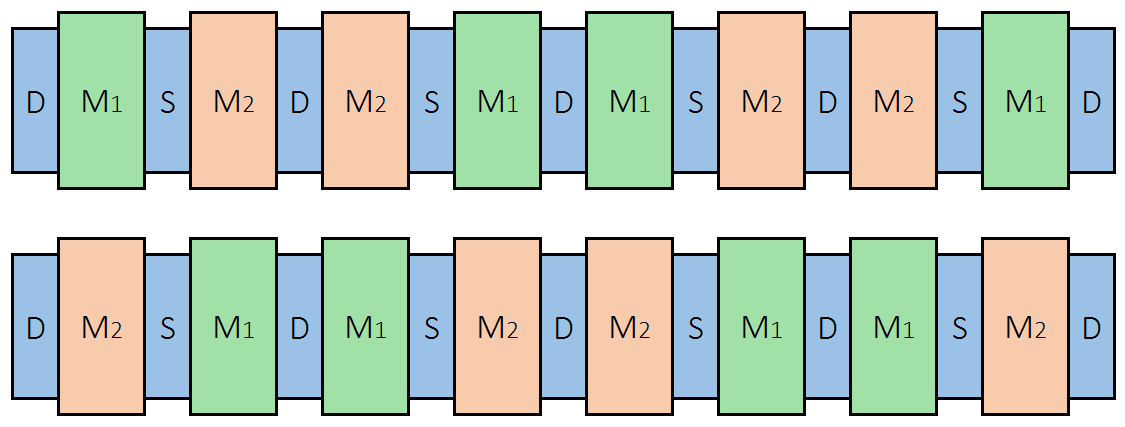
\includegraphics[keepaspectratio=true, scale=0.30]{teoricas/layout/cc2_2}
	\vspace{-0.5em}
	\caption{Estrutura resultante da agregação das difusões dos transístores.}
	\vspace{-0.8em} 
\end{figure}

Deve também ter-se em conta que a polarização foi feita ligando o \textit{guard ring} deste bloco ao \textit{guard ring} da estrutura \#1. Fica assim o bloco polarizado tal como foi explicado na secção anterior.

A implementação desta estrutura no Cadence é apresentada de seguida.

\begin{figure}[H]
	\centering
	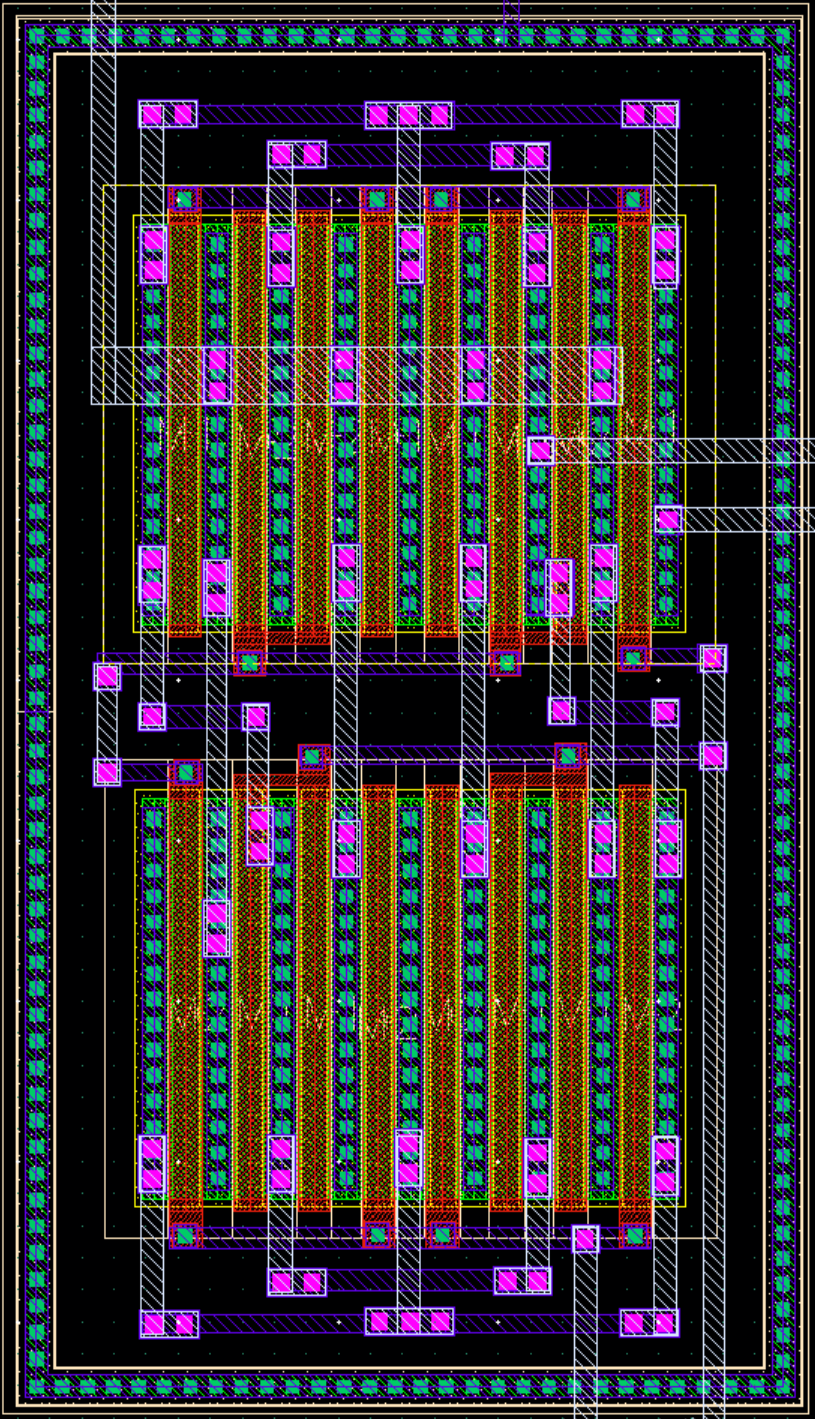
\includegraphics[keepaspectratio=true, scale=0.65]{exps/layout/pardiferencial}
	\vspace{-0.5em}
	\caption{\textit{Layout} da estrutura que corresponde ao par diferencial.}
	\vspace{-0.8em}
\end{figure}

\subsubsection{Estrutura \textit{common centroid} \#3}

 O ponto de partida para realizar o layout deste bloco foi organizar os transístores múltiplos de M\textsubscript{8} e M\textsubscript{7} cruzados de forma a garantir \textit{common centroid}. Como os transístores foram implementados com recurso a \textit{fingers} as difusões de cada um deles já se encontram sobreposta e, mais ainda, pode-se sobrepor as \textit{sources} de ambos, ficando o \textit{layout} com o aspecto que se segue.
 
\begin{figure}[H]
	\centering
	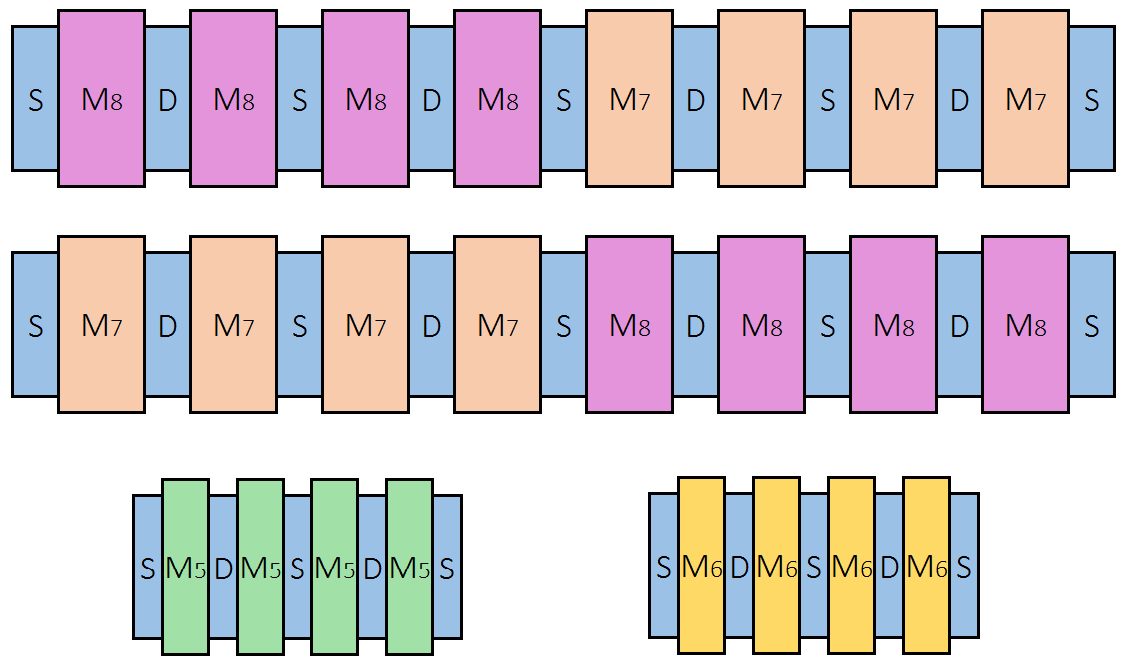
\includegraphics[keepaspectratio=true, scale=0.35]{teoricas/layout/cc3_1}
	\vspace{-0.5em}
	\caption{Esquema inicial do \textit{layout}.}
	\vspace{-0.8em} 
\end{figure}

Tem-se assim que este é um bloco bastante compacto e com as ligações entre transístores simples sendo as únicas prioridades prementes a utilização da menor área possível e garantir as regras de boas práticas relativamente aos troços de \texttt{Metal1} e \texttt{Metal2}.

Mais uma vez utilizou-se um \textit{guard ring} cuja função é proteger e polarizar o circuito tal como foi dito nos blocos anteriores. É feita então uma ligação entre este e o \textit{guard ring} do bloco \#1 ficando-se assim com a polarização feita a VDD, tal como desejado.

\begin{figure}[H]
	\centering
	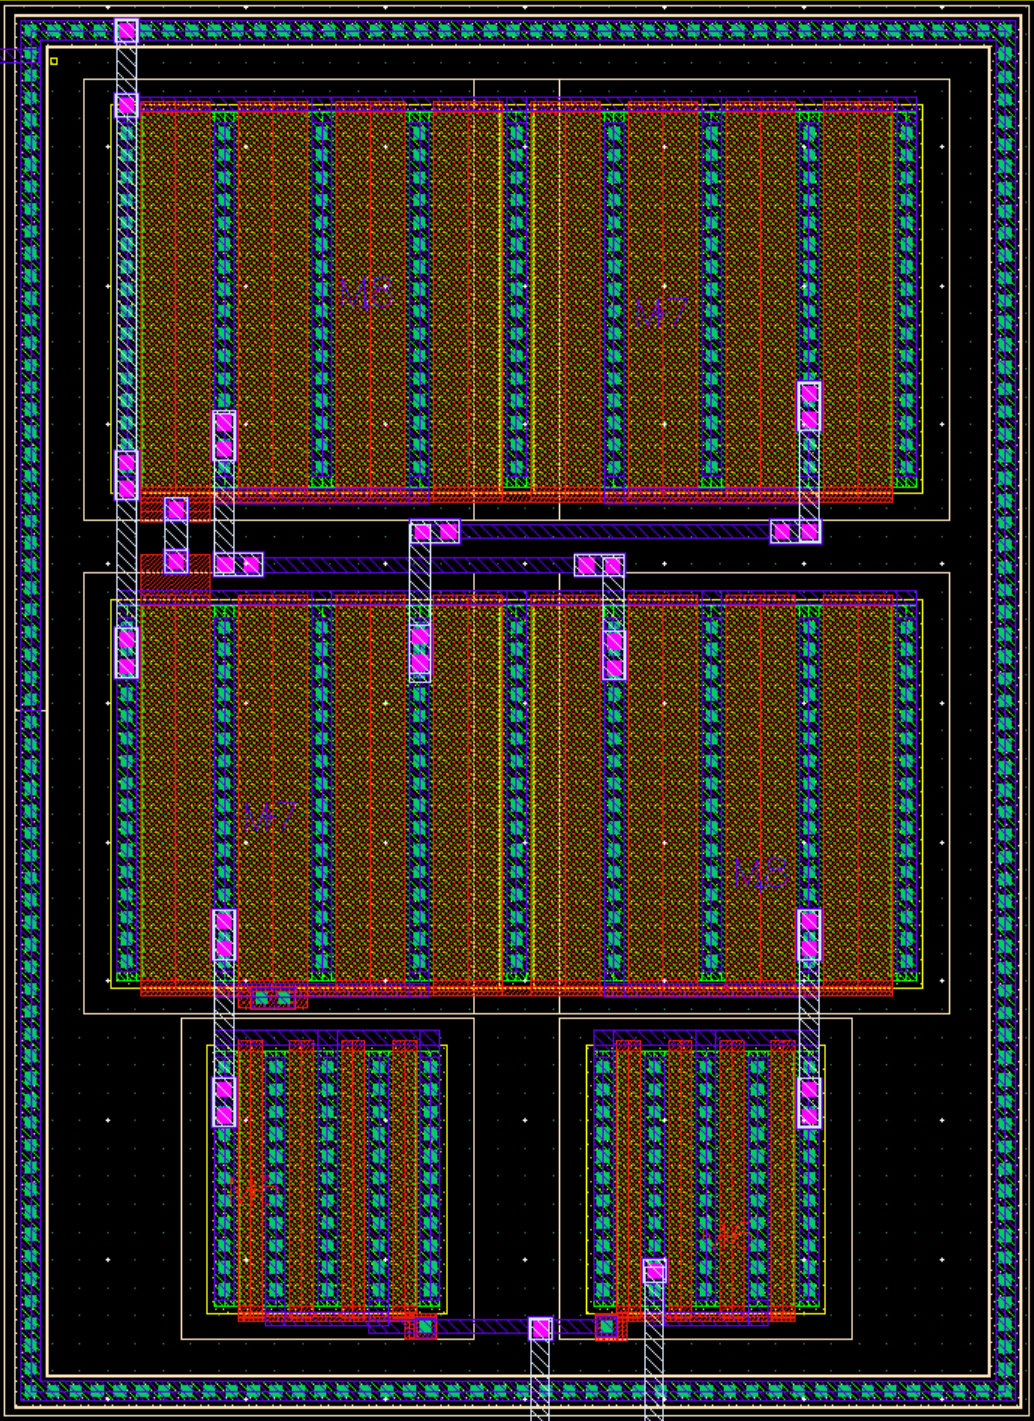
\includegraphics[keepaspectratio=true, scale=0.57]{exps/layout/espelhodecorrenteamp}
	\vspace{-0.5em}
	\caption{\textit{Layout} da estrutura que corresponde ao espelho de corrente cascode básico do tipo PMOS.}
	\vspace{-0.8em}
\end{figure}

\subsubsection{Estrutura \textit{common centroid} \#4}

Neste bloco estão presentes todos os transístores do tipo N o que levou a algumas dificuldades de organização dos transístores ao tentar obter-se uma estrutura \textit{common centroid} devidamente protegida de \textit{mismatches}. Começou-se então por colocar o número necessário de \textit{dummies} para que se obtivesse um bloco no qual todos os transístores observem as mesmas vizinhanças, como tem sido critério ao logo deste \textit{layout}. Obteve-se assim a seguinte estrutura.

\begin{figure}[H]
	\centering
	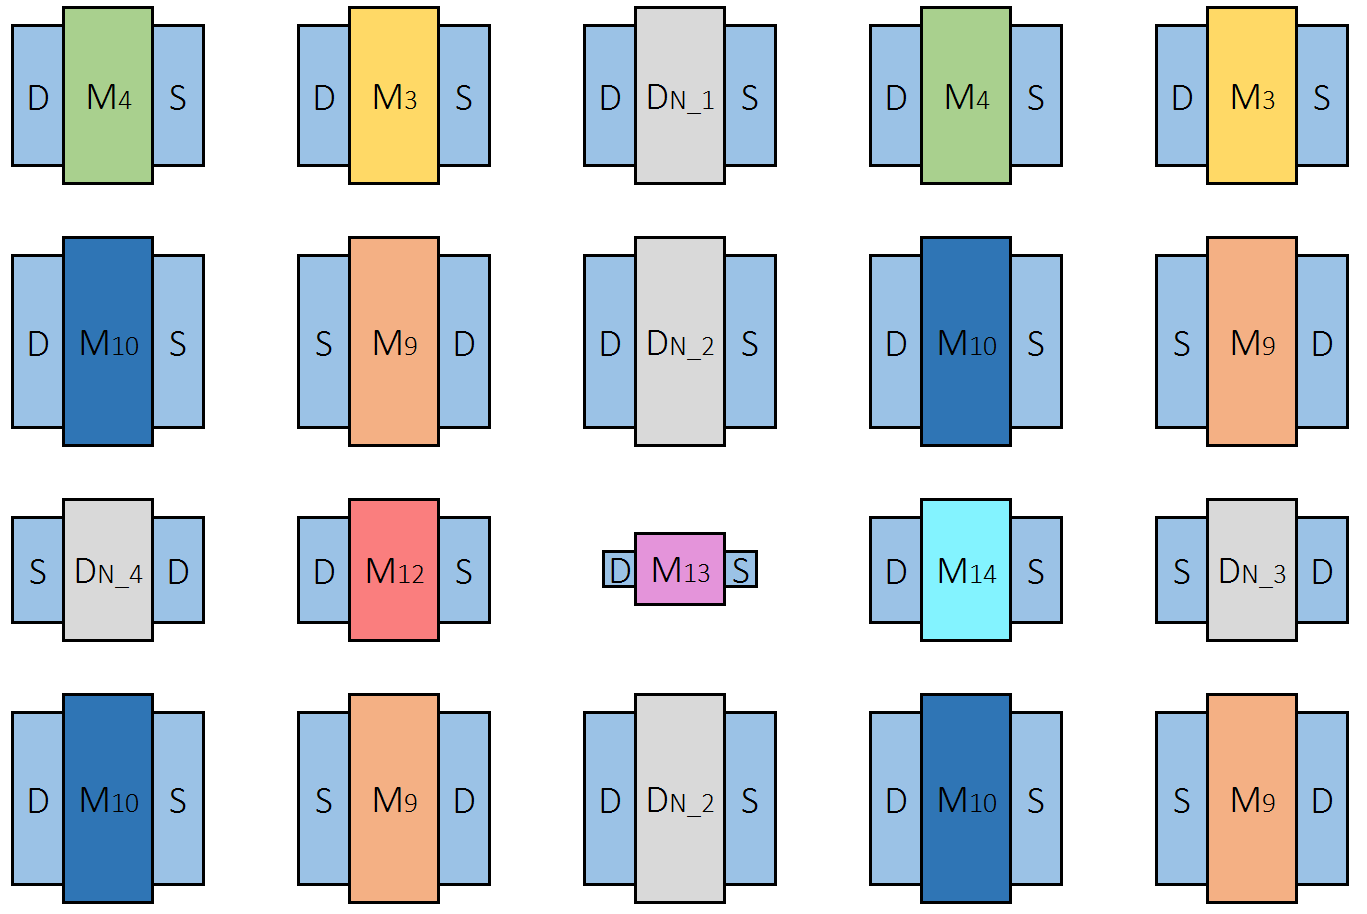
\includegraphics[keepaspectratio=true, scale=0.30]{teoricas/layout/cc4_1}
	\vspace{-0.5em}
	\caption{Esquema inicial do \textit{layout}.}
	\vspace{-0.8em} 
\end{figure}

Observou-se então que era possível sobrepor as \textit{sources} dos transístores M\textsubscript{9} e M\textsubscript{10} pelo que se reduziu as distâncias entre estes tanto quanto possível de forma a reduzir a área ocupada. Ficou-se assim como uma estrutura tal como se segue.

\begin{figure}[H]
	\centering
	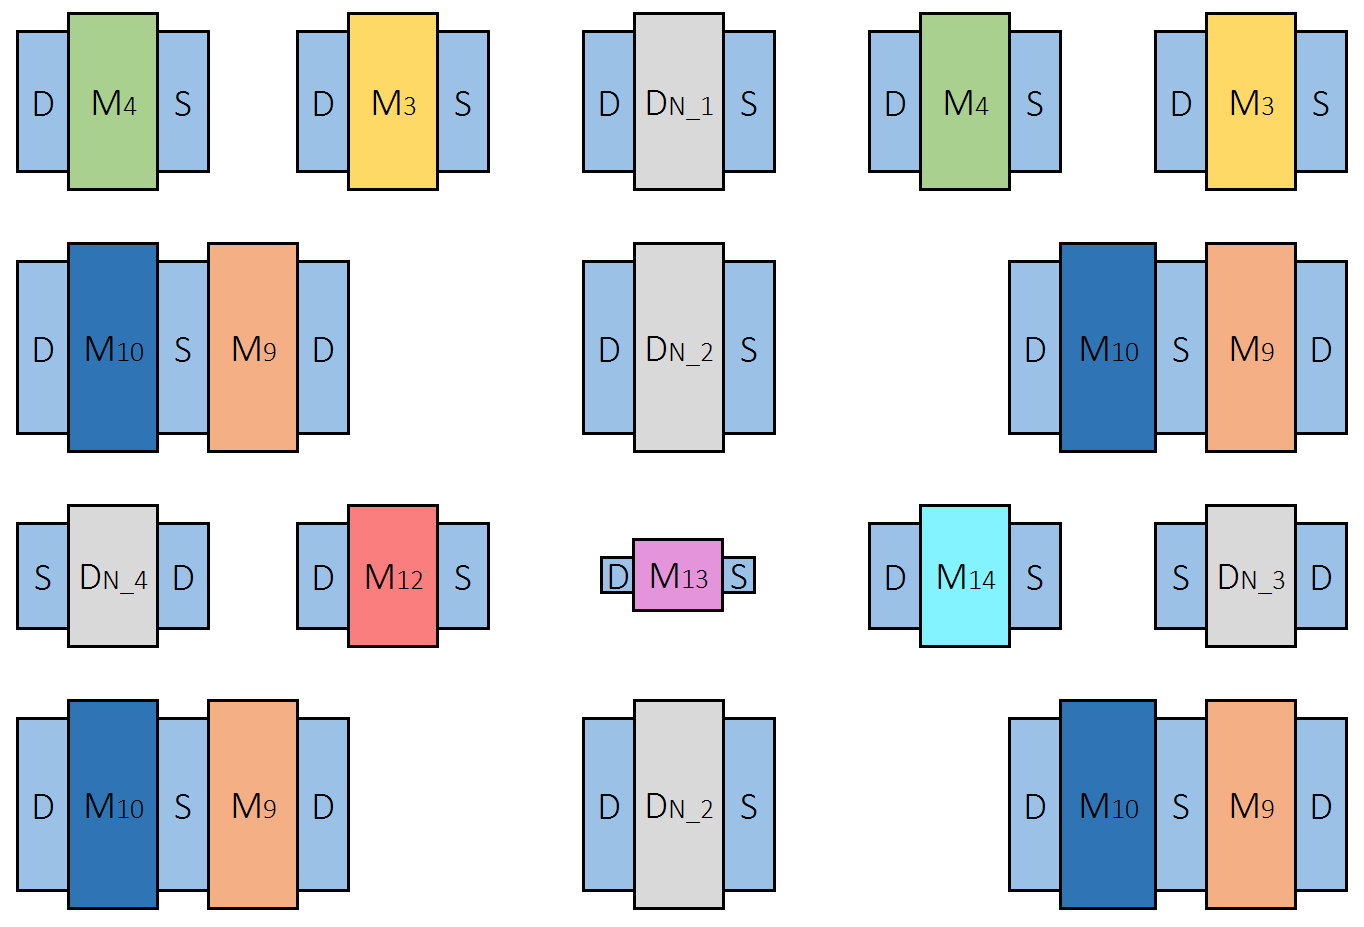
\includegraphics[keepaspectratio=true, scale=0.30]{teoricas/layout/cc4_2}
	\vspace{-0.5em}
	\caption{Estrutura resultante da agregação das difusões de alguns transístores.}
	\vspace{-0.8em} 
\end{figure}


Foram então feitas as ligações entre transístores garantindo as regras de boa prática, sempre que possível, assim como curto circuitar os \textit{dummies}. Neste caso, como se tratam de \textit{dummies} do tipo N, o curto circuito foi feito a GND, pois não se observa o mesmo problema que nos \textit{dummies} do tipo P, onde há o perigo de variações na fonte de tensão. Mais uma vez, como este se trata de um grupo apenas constituído por transistores NMOS, não foi necessária a utilização da máscara \texttt{NTUB}.

Por fim rodeou-se a estrutura com um \textit{guard ring} do tipo \texttt{pdiff\_sub}. Este \textit{guard ring} encontra-se ligado a GND polarizando-se assim o circuito e protegendo-o também de correntes de dispersão. 

\begin{figure}[H]
	\centering
	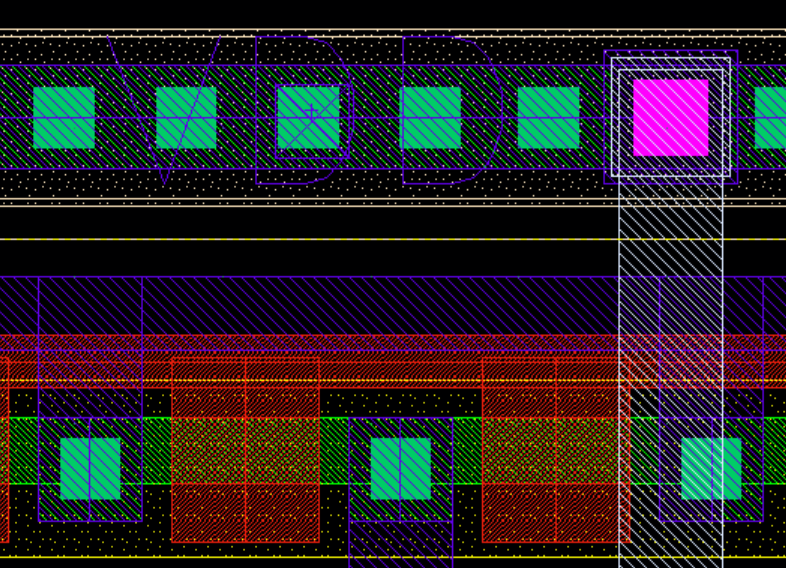
\includegraphics[keepaspectratio=true, scale=0.25]{exps/layout/pinVDD}
	\vspace{-0.5em}
	\caption{Colocação do \textit{pin} de GND sobre o \textit{guard ring}.}
	\vspace{-0.8em}
\end{figure}

\todo{imagem do pin do GND}

O resultado do \textit{layout} desta estrutura é assim o que se segue.

\begin{figure}[H]
	\centering
	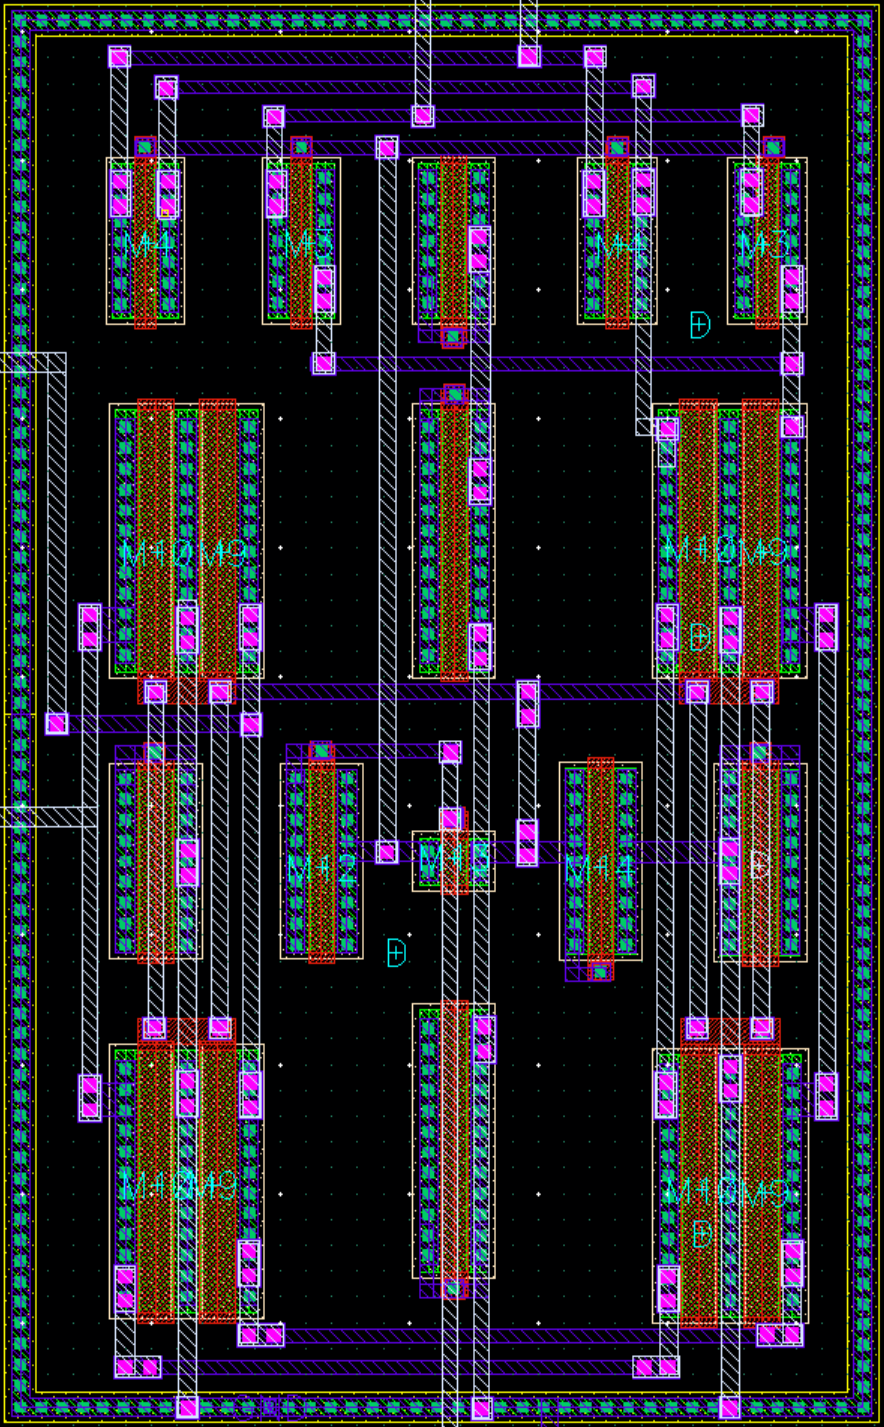
\includegraphics[keepaspectratio=true, scale=0.50]{exps/layout/nmos}
	\vspace{-0.5em}
	\caption{\textit{Layout} da estrutura que corresponde ao bloco de transístores NMOS.}
	\vspace{-0.8em} 
\end{figure}

\subsection{Ligações externas entre os blocos}

Após realizadas as ligações internas de cada bloco a tarefa que se segue é organizar estes de forma a ocupar o minimo de área possível assim como fazer as ligações entre estes.

Para realizar estas ligações entre blocos foi necessário ter especial atenção ao facto de que o material dos \textit{guard rings} é \texttt{Metal1} pelo que estas teriam que necessariamente ser feitas usando \texttt{Metal2} para evitar curto circuitos. 

Feitas estas ligações, de forma a proteger ainda mais o circuito colocou-se um \textit{guard ring}, polarizado a GND, em torno da forma final tal como se observa acima. Com esta polarização pode-se então fazer uma ligação por \texttt{Metal1} entre este e o \textit{guard ring} do bloco \#4 ficando assim também polarizado. Este \textit{guard ring} no entanto não é rectangular, tendo sido ajustado à forma do circuito final poupando-se ao máximo a área consumida. Neste \textit{guard ring} exterior foram também inseridos os restantes \textit{pins} de forma a que nenhum ficasse ``solto'' no meio so circuito.

Introduziram-se assim os \textit{pins} \texttt{In}, \texttt{Out}, \texttt{Vin+}, \texttt{Vin-}, \texttt{Ibias} e \texttt{Ibias2}. Como todos foram inseridos no \textit{guard ring} exterior são do material \texttt{Metal2} \texttt{Pin} sendo a sua \textit{label} do material complementar, ou seja \texttt{Pin} \texttt{Metal2}, tal como já mencionado anteriormente. Da mesma forma coloca-se um \textit{pin} para fazer a ligação a GND cujo material é \texttt{Metal1} \texttt{Pin} e a \textit{label} é \texttt{Pin} \texttt{Metal1}.

\todo{imagem dos pins}

O aspecto final do layout é assim o da imagem seguinte.

\begin{figure}[H]
	\centering
	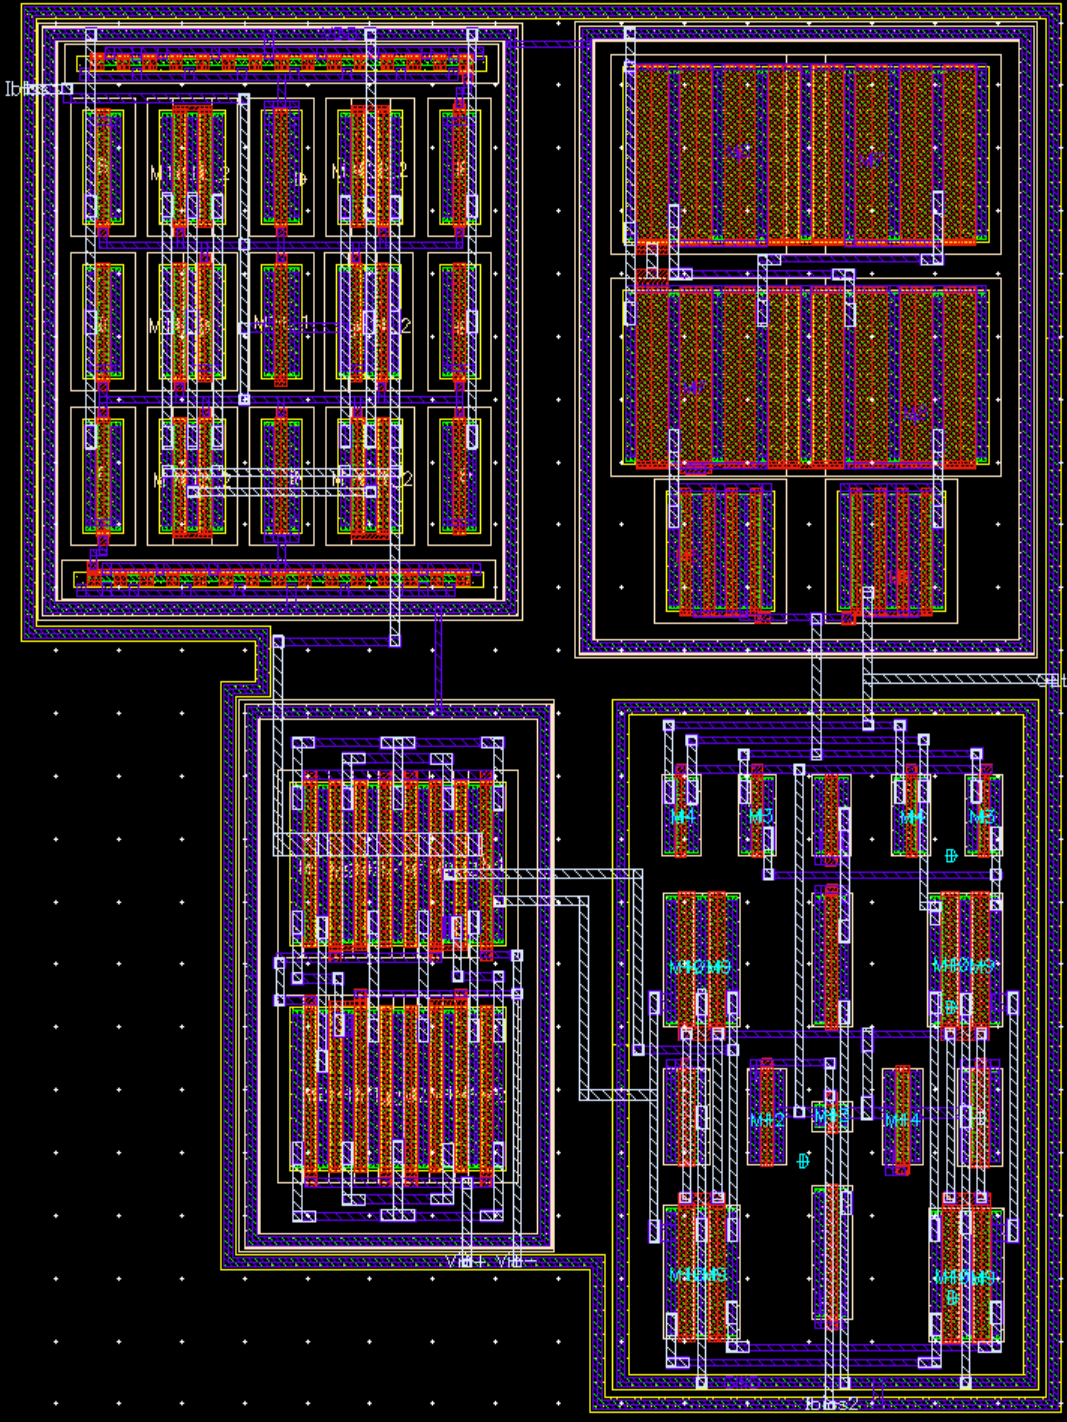
\includegraphics[keepaspectratio=true, scale=0.50]{exps/layout/full}
	\vspace{-0.5em}
	\caption{\textit{Layout} do circuito Cascode OTA.}
	\vspace{-0.8em} 
\end{figure}

Por fim calcula-se a área total do circuito usando as dimensões presentes na seguinte figura.

\begin{figure}[H]
	\centering
	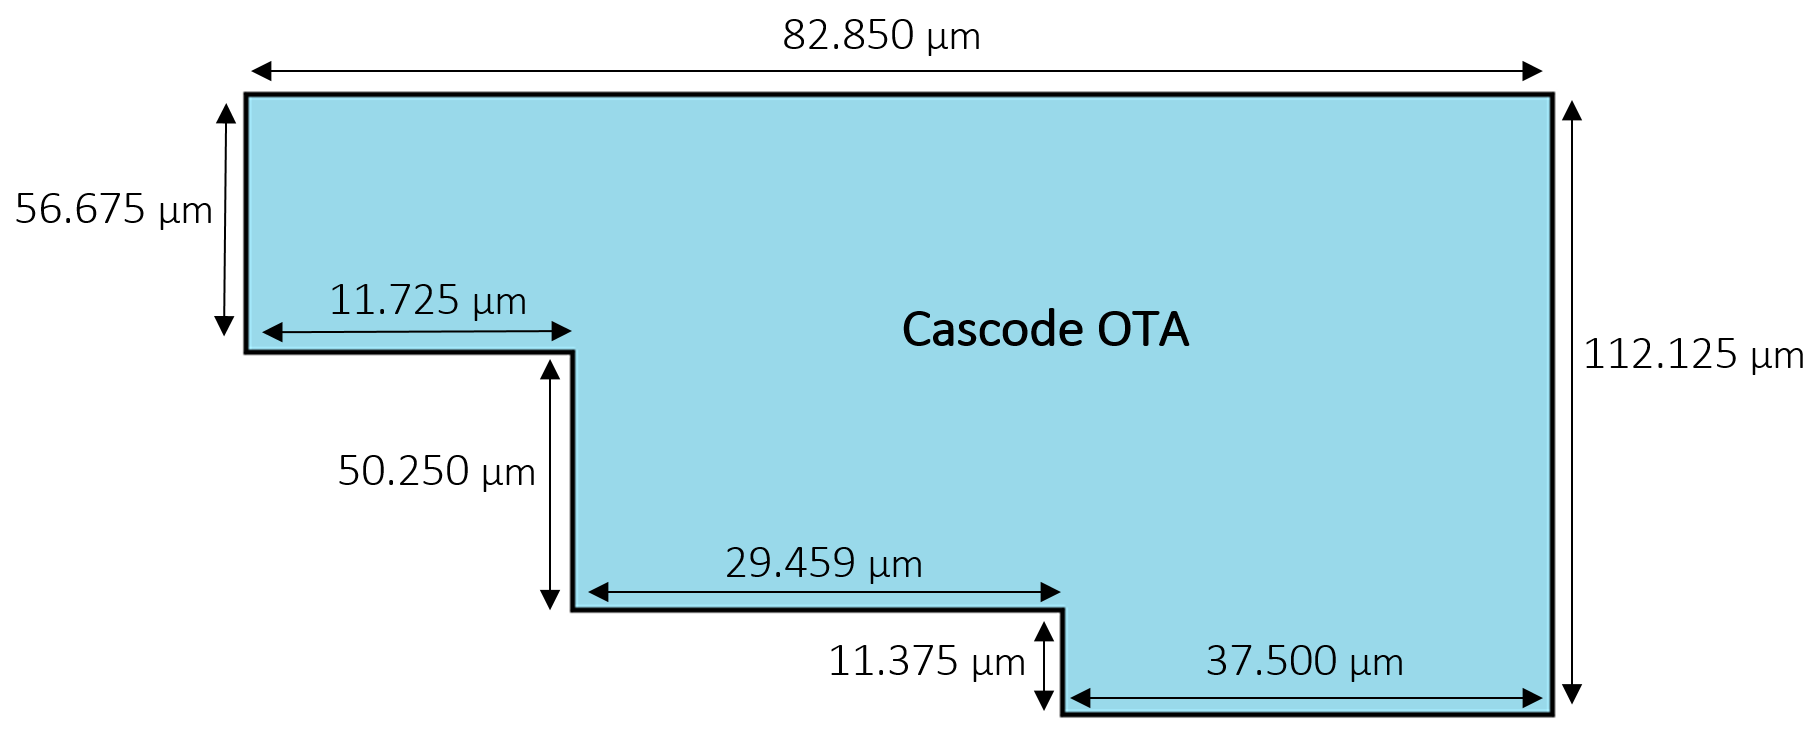
\includegraphics[keepaspectratio=true, scale=0.40]{teoricas/area}s
	\vspace{-0.5em}
	\caption{Dimensões para o cálculo da área.}
	\vspace{-0.8em} 
\end{figure}

\todo{calculo da área}

\section{Simulações com o circuito de \textit{layout}}

\subsection{Simulações de Monte Carlo e \textit{corners}}

Com o \textit{layout} feito seguiram-se então simulações de Monte Carlo e por \textit{Corners} para que se pudesse observar os efeitos das práticas e decisões tomadas ao longo da realização deste. Os resultados destas simulações apresentam-se então nas figuras seguintes.

\begin{figure}[H]
	\centering
	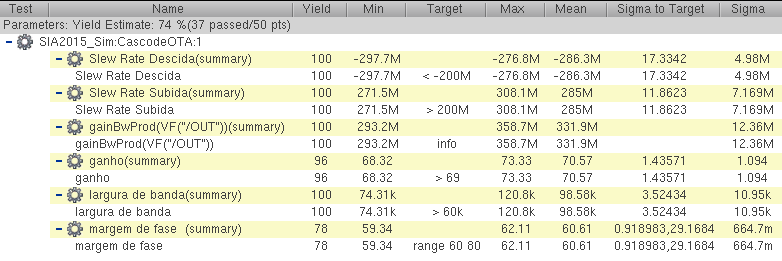
\includegraphics[keepaspectratio=true, scale=0.50]{exps/MonteCarlo_50pt_Novo_MultiTransistor_Layout}
	\vspace{-0.5em}
	\caption{simulação Monte Carlos para 50 pontos após realização do \textit{Layout}.}
	\vspace{-0.8em} 
\end{figure}

\begin{figure}[H]
	\centering
	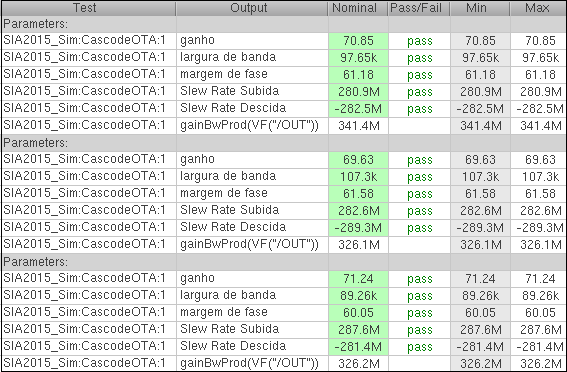
\includegraphics[keepaspectratio=true, scale=0.50]{exps/MonteCarlo_3pt_Novo_MultiTransistor_Layout}
	\vspace{-0.5em}
	\caption{Resultados obtidos para as 3 primeiras simulações de Monte Carlos após realização do \textit{Layout}.}
	\vspace{-0.8em} 
\end{figure}

\begin{figure}[H]
	\centering
	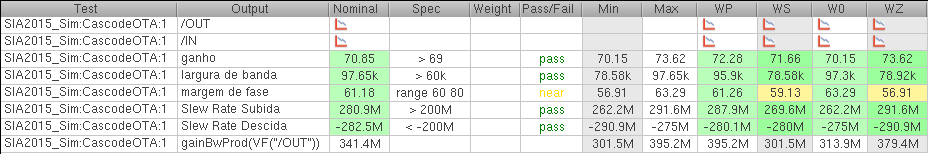
\includegraphics[keepaspectratio=true, scale=0.50]{exps/Corners_Novo_Layout}
	\vspace{-0.5em}
	\caption{Simulação por \textit{orners} após realização do \textit{Layout}.}
	\vspace{-0.8em} 
\end{figure}

Os resultados obtidos para a simulação de Monte Carlo são então, tal como esperado, melhores do que após a aplicação das técnicas de multiplicidade e \textit{fingers}, subindo o \textit{yeld} de 18\% para 74\%, sendo que o \textit{bottleneck} continua a ser a margem de fase.

Também na simulação por \textit{corners} os únicos resultados negativos foram na margem de fase, sendo que no entanto a situação melhora face ao caso após  a aplicação de multiplicidade e \textit{fingers}.

\todo{há alguma desculpa a dar para os maus resultados da fase ou aceitamos este yeld?}

\todo{tabela do enunciado}

\subsection{Substituição do amplificador do SAR ADC}

\todo{substituir initial target}

\pagebreak

\section{Conclusões}

Para o \textit{final target} deste projecto houve dois objectivos - corrigir os erros encontrados no \textit{middle target} após realizar as simulações Monte Carlo e de \textit{corners} e também fazer o \textit{layout} do circuito final.

Partindo do \textit{middle target} correu-se então a simulação de Monte Carlo e os valores obtidos foram inferiores aos expectáveis pelo que houve necessidade de se fazer alterações às dimensões de alguns dos transístores, assim como corrigir as expressões que estavam a ser utilizadas para calcular a \textit{slew rate}. Em grande parte o parâmetro que teve que sofrer a maior correcção foi a margem de fase e o ganho pelo que as alterações foram feitas nos pares de transistores M\textsubscript{7}/M\textsubscript{8} e M\textsubscript{3}/M\textsubscript{4}, assim como alguns ajustes finos nos restantes transístores.

Feitas estas alterações e com resultados muito melhores procedeu-se então ao \textit{layout}. De forma a realizar o \textit{layout} começou-se por aplicar as técnicas de multiplicidade e \textit{fingers} protegendo-se o circuito de \textit{mismatches}. Para este efeito foram também utilizados \textit{dummies} para que se tenha as mesmas vizinhanças em todos os transístores, e garantir que as estruturas são \textit{common centroid}. As ligações foram feitas tentando obedecer à regra de boa prática de utilizar \texttt{Metal1} para troços na vertical e \texttt{Metal2} para troços na horizontal, violando-a apenas de forma a evitar grandes aumentos de área ou curto circuitos que não eram pretendidos. De forma a proteger o circuito de correntes de dispersão assim como para polarização colocaram-se \textit{guard rings} em torno de cada bloco individual assim como do circuito final.

Ao longo de todas estas alterações foram feitas simulações Monte Carlo e de \textit{corners} observando-se os efeitos de cada passo para que se obtivessem os requisitos finais do \textit{target}.

\todo{explicar a parte do ENOB}

Observa-se assim que os requisitos foram, na sua grande maioria, cumpridos com sucesso e deu-se o trabalho por concluído.

Com este \textit{final target} obteve-se assim experiência relativamente às boas práticas e à forma como se deve proceder na realização de um \textit{layout}.

\end{document}